%
% Unless otherwise indicated, the copyright in this material is 
% owned by Joerg Evermann. This material is licensed to you under the 
% Creative Commons by-attribution non-commercial license (CC BY-NC 4.0)}
%
\section*{Learning Goals}

After reading this chapter, you should be able to:
\begin{itemize}
  \item List and describe the primitive data types of numbers, characters and strings, dates and times, and the standards and options for their representation or serialization.
  \item Characterize and differentiate among structured data types in R and Python, such as lists, vectors, sets, etc. 
  \item List and describe structured data, such as tables, documents, and graphs, including standardized serialization and exchange formats.
  \item List and describe unstructured data formats and identify use cases in business analytics. For text data, be able to apply regular expressions and string edit distances for basic text analysis.
  \item Identify relevant questions to ask with respect to the quality of a data set. Describe the importance of data provenance in ensuring data quality.
  \item Describe the process and different activities for data cleaning, that is, for improving data quality.
  \item Identify useful external data sources. 
\end{itemize}

\section{Introduction}

Business analytics is the use of data for understanding, description, prediction, prescription and decision making. Hence, it is important to understand the different types of data and the variety of formats in which they can exist. 

This section first introduces primitive data types, such as numbers and text. There are many complexities to be aware of that can make analytics challenging. Next, complex data types are introduced, such as tables, documents, and graphs, which are useful in describing complex information, such as customer purchase history in tables, product descriptions in documents, or supply chain logistics in a graph. Then, unstructured data in the form of text, images, and audio/video information is explained. Data in these formats may be market information from financial reports (text), quality control photos taken on a manufacturing line (images), or video captured inside the chemical reactors of an oil refinery.

In the second section, you will learn about data quality, data cleaning, and data provenance. It is important to understand potential problems with the data you use, how to identify them, and how to address them. Data provenance, that is, understanding where the data was collected or created, and how it was processed, is important because errors or biases may be introduced at various stages of the processing and handling pipeline.

The final section introduces different sources data sources. While most data for business analytics is internally produced by an organization, there is a vast amount of external information available to use and to combine with internal data for richer business analytics. 

\section{Data Types}

\subsection{Primitive Types}

Primitive data types are basic types of data built into programming languages and other software systems such as statistics and analytics tools. They represent the simplest forms of data and serve as the building blocks for constructing more complex data structures.

\begin{table}
\renewcommand{\arraystretch}{1.25}

\begin{tabularx}{\textwidth}{l|X} \hline
char 			& Individual Characters\\
string			& A string of characters\\
byte			& 1 byte, $-128 \ldots 127$ or one ASCII characters \\
int (16 bit)	& ''Short'', Integer numbers, $-32,768 \ldots 32,767$ \\ 
int (32 bit)	& ''Long'', Integer numbers, $-2,147,483,648 \ldots 2,147,483,647$ \\
int (64 bit)	& Integer numbers, $-9,223,372,036,854,775,808 \ldots$ $9,223,372,036,854,775$ \\
float			& Decimal numbers, 6 to 7 significant digits, ''single precision'' \\
double			& Decimal numbers, 15 to 16 significant digits, ''double precision'' \\
boolean			& Logical, true/false, 1 or 0 \\ \hline
\end{tabularx} 
\caption{Primitive Data Types}
\label{tab:primitive}
\end{table}

Table~\ref{tab:primitive} shows a list of common data types. However, not all software systems use the same names, and not all systems make the same distinctions. For example, the R system uses the terms \texttt{numeric} (which is actually a double type) and \texttt{integer} (which is a 32 bit integer).

Additionally, it is important in statistics and analytics to indicate the lack of a value, that is, a ''missing value''. Different systems use different special names for this. The R statistical system uses the term ''\texttt{NA}'', while the Python programming languages uses ''\texttt{None}'' and the SQL database language uses the term ''\texttt{Null}''. Moreover, the meaning of these in practice can be ambiguous and says nothing about the reason for the missingness. For example, is the value not appropriate to the thing measured (e.g. in a table of geometric objects, the diameter value is simply not appropriate for two-dimensional object)? Was it missed during data collection? Was it withheld during data collection? Was it removed during initial analysis as an outlier?

\subsubsection*{Numbers} 

As Table~\ref{tab:primitive} indicates, decimal numbers can be represented using different numbers of bytes with different precisions. Integer numbers are relatively straightforward\index{Integer}. Here, a number is simply represented as its equivalent \emph{binary number}\index{Binary number} (base 2, with digits 0 to 1), often with the first bit indicating the sign (positive/negative).

To represent decimal numbers, computers use the floating point representation\index{Floating point number} defined by the IEEE 754 standard\footnote{\url{https://en.wikipedia.org/wiki/IEEE_754}}. Figure~\ref{fig:ieee754} shows how decimal numbers are represented in binary form. A \texttt{float}, or single precision number occupies 4 bytes (32 bits): 1 bit for the sign, 8 bits for an exponent, and 23 bits for the fraction (also called ''significand'' or ''mantissa''). With this, a \texttt{float} has a precision of approximately 6 to 7 decimal digits and a range at full precision between $\pm 1.18 \times 10^{-38}$ \ldots $\pm 3.4 \times 10^{38}$. 

\begin{figure}[h]
\centering
\begin{subfigure}[t]{\textwidth}
\centering
\includegraphics[width=.9\textwidth]{ieee75432.png}\\ \vspace{5mm}
\scriptsize{\url{https://commons.wikimedia.org/wiki/File:Float_example.svg}}
\caption{32 bit float}
\end{subfigure}
\begin{subfigure}[t]{\textwidth}
\centering
\includegraphics[width=\textwidth]{ieee754.png}
\scriptsize{\url{https://commons.wikimedia.org/wiki/File:IEEE_754_Double_Floating_Point_Format.svg}}
\caption{64 bit double}
\end{subfigure}
\caption{Floating Point Numbers (IEEE 754 Standard)}
\label{fig:ieee754}
\end{figure}

A \texttt{double}, i.e. a double precision number, occupies 8 bytes (64 bits): 1 bit for the sign, 11 bits for an exponent and 52 bits for the fraction. It has a precision of 15 to 16 decimal digits and a range at full precision between $\pm 2.23 \times 10^{-308}$ \ldots $\pm 1.80 \times 10^{308}$. 

\subparagraph*{Example:} Consider the number 0.15625 in the top of Figure~\ref{fig:ieee754}. Its IEEE 754 float representation can be understood as follows:
\begin{enumerate}
	\item First, convert $0.15625$ to binary, which is $0.00101_2$ ($1/8+1/32$).
	\item Rewrite in normalized scientific notation: $1.01_2 \times 2^{-3}$.
	\item Sign Bit: 0.15625 is positive, so the sign bit is 0.
	\item Exponent: The actual exponent is $-3$, and the biased exponent is $-3+127=124$, which is $01111100_2$ in binary.
	\item Fraction (significand, mantissa): The fraction is the normalized value without the leading 1, so it is $010000000000000000000000_2$ (23 bits).
\end{enumerate}

Combining these components as shown in Fig.~\ref{fig:ieee754} leads to the number ''01011111 00010000 00000000 00000000'', written in 4 bytes of 8 bits each.

While the IEEE 754 standard defines how computers store decimal numbers internally, when exchanging information, numbers are printed as plain text. Such ''printing as plain text'' is called ''\emph{serialization}'', because the data are written as a series of characters or bytes. Writing out decimal numbers is fraught with complexities due to different idiosyncratic styles of writing or formatting numbers, depending on the application or the locale (that is, the dominant rules in the location of the user). 

\begin{table}[h]
\renewcommand{\arraystretch}{1.25}
\centering

\begin{tabular}{r|l} \hline
\textbf{Format} & \textbf{Comment} \\ \hline
-1023476.56 & \\
-1023476,56 & some locales use comma as decimal separator \\
-1,023,476.56 & some locales use comma for grouping \\
-1.023.475,56 & some locales use comma as sep and points to group \\
(1,023,476.56) & some applications use brackets for negation \\
-1 023 476.56 & some locales use space for grouping \\
-1.02347656e+06 & ''scientific notation'' \\
-1023.47656e+03 & also ''scientific notation'' \\ \hline
\end{tabular}
\caption{Serializing Numbers to Text}
\label{tab:floatingpointtext}
\end{table}

The most frequent variations occur with respect to the decimal point (some locales, for example in Europe, use a comma instead), the grouping of digits (some locales group thousands, millions, etc. with spaces, points, commas, and other characters), writing negative numbers (in accounting, negatives are often put in parentheses instead of using a minus sign), and ''scientific notation'', which specifies numbers as coefficients and exponent for powers of 10 (for example $1.234e+3 = 1.234 \times 10^3 = 1234$; $1.234e-2 = 1.234 \times 10^{-2} = 0.01234$). Table~\ref{tab:floatingpointtext} shows examples of some idiosyncratic ways of writing the same number. 

\begin{tcolorbox}[colback=alert]
It is important to verify the number format in any data set, and to transform it into one that is readable and usable by the chosen business analytics tool. 
\end{tcolorbox}

\subsubsection*{Characters \& Strings}

There exist a multitude of writing systems beyond the Latin alphabet, using many different symbols. Symbols can represent consonants, consonant-vowel sequences, phonemes, words or morphemes, or syllables, leading to a vast range of symbols across the written languages of the world. 

\begin{wrapfigure}{l}{1in}
\begin{center}
\includegraphics[height=.5in]{unicode.png}
\end{center}
\end{wrapfigure}

The Unicode system\footnote{\url{https://home.unicode.org/}}\index{Unicode} was developed to address the limitations of earlier encoding systems and to enable consistent, universal representation of text from all the world's writing systems. Before Unicode, there were different encoding systems, such as ASCII (American Standard Code for Information Interchange), which could only represent a limited set of characters (primarily used in the English language). This led to difficulties in representing text in languages with larger character sets or different scripts. The Unicode Consortium was founded in 1988 and incorporated in 1991 with the goal of developing a universal character encoding standard. Unicode was standardized in 1998 as ISO/IEC standard 10646 and its popular UTF-8 encoding was standardized as RFC 2279\footnote{\url{https://datatracker.ietf.org/doc/html/rfc2279}}. Over the years, Unicode has been expanded and refined to include a wider array of characters, symbols, and scripts. This includes not only modern languages but also historic scripts, mathematical symbols, emojis, and more. By providing a unique identifier for every character, regardless of the computer system, software application, or programming language, Unicode solves the problem of inconsistent encoding and ensures that text appears consistently across different systems and devices. It has become the standard for modern software and internet protocols and  is fundamental for web content, databases, applications, and more. The latest version of Unicode as of this writing (v15.1) contains 149,813 characters for different 161 scripts, including 3782 emojis\footnote{\url{https://www.unicode.org/versions/stats/}}. 

UTF-8 (Unicode Transformation Format -- 8-bit)\index{UTF-8}\index{Unicode transformation format} is the most common method for representing Unicode characters. It uses between one and four bytes to represent a character and is backwards compatible with ASCII because the initial 127 Unicode characters are identical to the corresponding ASCII characters. 

\subparagraph*{Example:} Consider the word ''Inuktitut''. This word is written in the Inuktitut writing system as 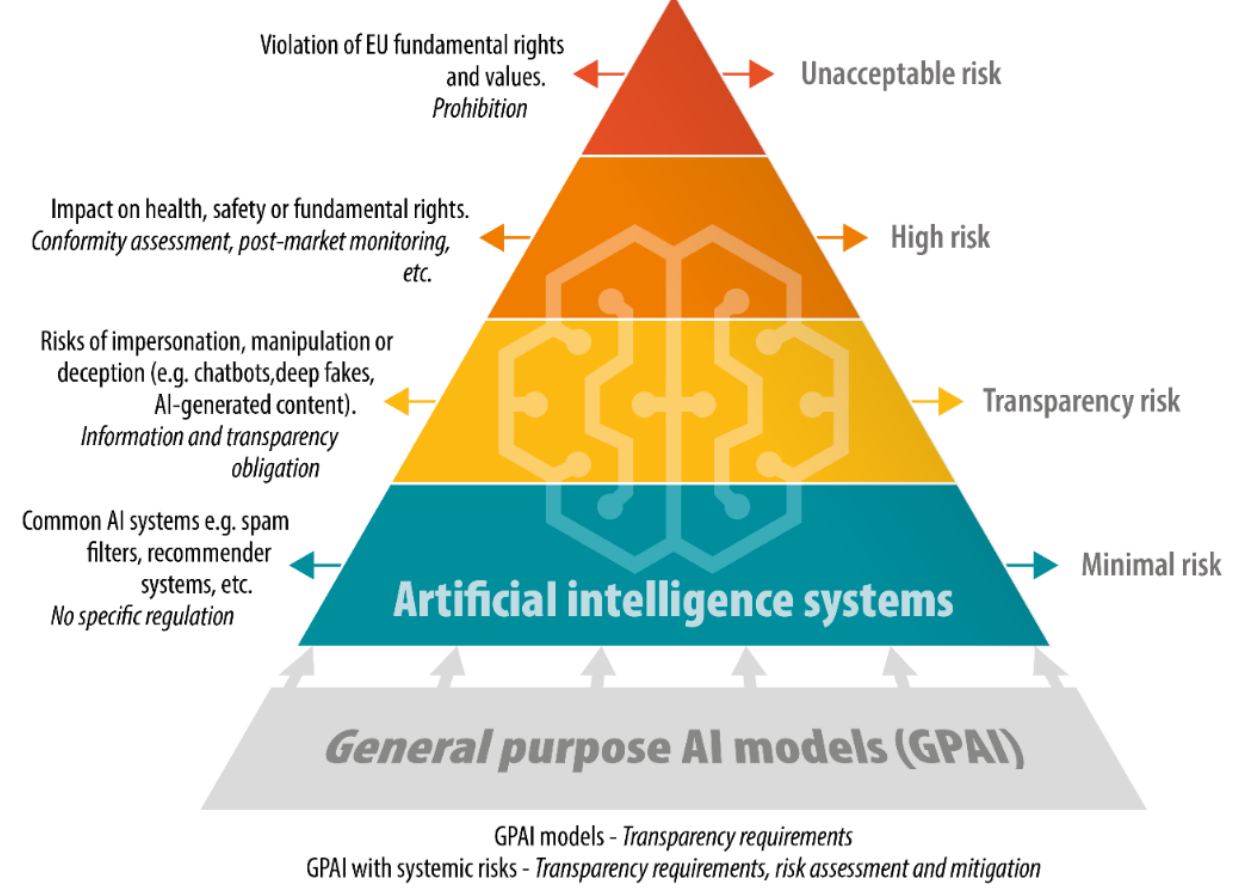
\includegraphics[height=1.5\fontcharht\font`\B]{screen2.png}, which contains six symbols (the Inuktitut writing system is not alphabetic, it is syllabic)\footnote{Using \url{https://www.inuktitutcomputing.ca/Transcoder/index.php} and \url{https://www.compart.com/en/unicode/}}. The corresponding Unicode character numbers (''codepoints'') are: U+1403, U+14C4, U+1483, U+144E, U+1450, U+1466. These are given as \emph{hexadecimal numbers}, using a base of 16 with digits from 0 to F. In text documents this may be written as \textbackslash u1403 \textbackslash u14c4 \textbackslash u1483 \textbackslash u144e \textbackslash u1450 \textbackslash u1466 when the document is read/parsed by an appropriate software tool that can understand this way of writing Unicode characters. 

The corresponding decimal (base 10, with digits from 0 to 9) Unicode character numbers are 5123, 5316, 5251, 5198, 5200, 5222. These are used when the text is written for web content in HTML as HTML entities, such as ''\&amp;\#5123; \&amp;\#5316; \&amp;\#5251; \&amp;\#5198; \&amp;\#5200; \&amp;\#5222;''.

Using UTF-8, each of these six characters can be encoded in 3 bytes. These are usually written in hexadecimal form, indicated by the ''0x'' prefix. Hexademical form is a base 16 system and uses ''numbers'' between 0 and F, that is, it uses 0, 1, 2, 3, 4, 5, 6, 7, 8, 9, A, B, C, D, E, and F as numbers. For example, 0xE1 is 14 (the ''E'') times 16 (the first digit) + 1 times 1 (the second digit), yielding 225. 0x. 

The sequence of Unicode characters for the word ''Inuktitut'' becomes 0xE1 0x90 0x83 (first symbol) 0xE1 0x93 0x84 (second symbol) 0xE1 0x92 0x83 (third symbol) 0xE1 0x91 0x8E (fourth symbol) 0xE1 0x91 0x90 (fifth symbol) 0xE1 0x91 0xA6 (sixth symbol). 

As a business analyst, you may come across data that contains Unicode characters either spelled out in the ''\textbackslash uXXXX'' form, or UTF-8 encoded in byte sequences, or in the HTML format. While you do not need to understand the technical details of Unicode and its different encodings, you should be aware that data in this format is common and you need to know how to deal with it when you encounter it. This includes using a Unicode-aware data storage and management system, using a Unicode-aware business analytics tool, and using a Unicode-aware visualization or report-writing tool.

\begin{tcolorbox}[colback=code]
\subsubsection*{Hands-On Exercise}
\begin{itemize}
	\item Choose your favourite emoji
	\item Determine its Unicode number (''codepage'')
	\item Determine its UTF-8 encoding
\end{itemize}
\end{tcolorbox}

\subsubsection*{Dates and Times}

The world has largely standardized on the Gregorian calendar for secular and commercial use, while other calendar systems exist now only for religious or traditional purposes. However, as with written numbers, written dates show a bewildering variety of forms, depending on the locale and other traditions.

Complexities are introduced by 12 hour (AM/PM) versus 24 hour time formats (''14:30'' is ''2:30PM''), different time zones across the world, leap seconds and leap years, week numbering (does it start with the first full week?), different written formats for the sequence of days, months, and years (is ''06-07-09'' June 7, 2009 or July 6, 2009, or July 9, 2006?), different separators between years, dates, and months (''06/07/09'' and ''06-07-09''), and the difficult arithmetic when using years, months, and days. 

The ISO 8601\footnote{\url{https://en.wikipedia.org/wiki/ISO_8601}} (first published in 1988) and RFC 3339\footnote{\url{https://datatracker.ietf.org/doc/html/rfc3339}} (published in 2002) standards define how dates\index{Date} and times\index{Time} should be written. Table~\ref{tab:iso8601} shows a summary of the ISO 8601/RFC3339 rules (the italicized forms are in ISO 8601 but not in RFC 3339). However, these standards are by no means universally accepted and reading/parsing date and time data remains a difficult and complex task in many business analytics settings. 

Even within the ISO 8601 standard, there are numerous ways to express the same date or time, such that June 13, 2024 can be written as an ordinal date (''2024-165'') or a week date (''2024-W24-4'') and the time of T13:45:30 can be written as ''T13:45.500'' or as ''T1345.500''. 

\begin{tcolorbox}[colback=alert]
For a business analyst, it is important to verify the format of dates and times in any data set, especially when the data comes from different or external sources.
\end{tcolorbox}

\begin{table}
\centering
\renewcommand{\arraystretch}{1.25}

\begin{tabular}{l|l} \hline
	Calendar dates & YYYY-MM-DD  \\ \hline
	\textit{Ordinal dates} & \textit{YYYY-DDD} \\ \hline
	\textit{Week dates} & \textit{YYYY-Www-d} \\ \hline
	\multirow{5}{*}{Times} & Thh:mm:ss.sss \textit{(or Thhmmss.ss)} \\
	& Thh:mm:ss \textit{(or Thhmmss)} \\
	& \textit{Thh:mm.mmm or Thhmm.mmm} \\
	& \textit{Thh:mm or Thhmm} \\
	& \textit{Thh.hhh} \\ \hline
	\multirow{2}{*}{Time Zones} & <time>Z or <time>$\pm$hh:mm or \\
	& \textit{(<time>$\pm$hhmm or <time>$\pm$hh)} \\ \hline
	Combined & <date>T<time> \\
	Periods & PnYnMnDTnHnMnS or P<date>T<time> \\ \hline
\end{tabular} \\ \vspace{.5\baselineskip}

\small The \textit{italicized} forms are in ISO 8601 but not in RFC 3339
\caption{ISO 8601 / RFC 3339 Rules for Dates and Times}
\label{tab:iso8601}
\end{table}

\begin{tcolorbox}[colback=alert]
A year is a leap year if it can be divided by four and (cannot be divided by 100 but can be divided by 400). Formally: \\
\small
\texttt{(year \% 4 == 0) and (year \% 100 != 0 or year \% 400 == 0)}
\normalsize
\end{tcolorbox}
 
\begin{tcolorbox}[colback=code]
\paragraph*{Hands-On Exercise} 

\textit{\textbf{\vspace{3mm} \\The territory of Nunavut was created on April 1st, 1999. \vspace{3mm}}}

\begin{itemize}
	\item Express the date in RFC 3339
	\item Calculate the number of days since the creation of Nunavut
	\item Assume that a ceremony took place at 3PM that day in Iqaluit and express this date-time in RFC 3339
	\item Assume the ceremony lasted for 125 minutes and express this duration in RFC 3339
\end{itemize}
\end{tcolorbox}

\subsubsection*{Collections}

Collections\index{Collection (data type)} can store multiple instances of primitive data, often heterogeneous. Different collection types have different characteristics in terms of whether they are 

\begin{itemize}
\item ordered or unordered, 
\item homogeneous (same primitive types) or heterogeneous (different primitive types), 
\item unique or allow duplicates, 
\item mutable (can be changed) or immutable (cannot be changed). 
\end{itemize}

Different software tools offer different kinds of structured types and unfortunately the terminology is not necessarily consistent across software tools. Table~\ref{tab:structured} provides a summary of structured types in Python and R, with examples and key characteristics of the type.

\begin{table}
\renewcommand{\arraystretch}{1.25}
\footnotesize
\centering

\begin{tabular}{l|l|l} \hline
\multicolumn{3}{c}{\textbf{Python}} \\ \hline
list\index{List (in Python)} & \texttt{[1, 2, "a", "b", 2]} & mutable, ordered \\
tuple\index{Tuple (in Python)} & \texttt{(1, 2, "a", "b", 2)} & immutable \\
set\index{Set (in Python)} & \texttt{\{1, 2, "a", "b"\}} &  mutable, unordered, unique \\
dict\index{Dictionary (in Python)} & \texttt{\{"make": "Ford", "year": 2023\}} & mutable \\ \hline
\multicolumn{3}{c}{\textbf{R}} \\ \hline 
list\index{List (in R)} & \texttt{list(1, 2, "a", "b", 2)} & mutable, ordered \\
vector\index{Vector (in R)} & \texttt{c(1, 2, 3)} & mutable, same primitive type \\
factor\index{Factor (in R)} & \texttt{as.factor(c("Hot", "Med", "Cold"))} & ordered\\
matrix\index{Matrix (in R)} & \texttt{matrix(c(1, 2, 3, 4), nrow=2)} & \\
array\index{Array (in R)} & \texttt{array(c(1, 2, 3), c(4, 5, 6))} \\ \hline
\end{tabular}
\caption{Structured data types (''collection types'') in Python and R}
\label{tab:structured}
\end{table}

\FloatBarrier
\subsection{Structured Data}

Data that you encounter in business analytics is built on the primitive and collection data types described in the previous section. We distinguish between structured data, such as tables, key-value pairs, documents, or graphs, and unstructured data, such as text, images, and audio/video data. The latter are called unstructured because these data essentially come as simply a sequence of characters or bytes. Information must first be identified in them and extracted from them, before it can be used for analytics. 

\subsubsection*{Tables}

Table data\index{Table} refers to a method of organizing data in a structured, tabular format, where the data is arranged in rows and columns. Each \emph{row} in a table represents a single record or entry. For instance, in a table of customer data, each row could represent a different customer. \emph{Columns}, sometimes called \emph{fields}, represent different attributes or characteristics or features of a record. In the customer data example, columns might represent attributes of a customer such as their name, address, and purchase history. The intersection of a row and a column is called a cell. Each \emph{cell} contains a single piece of data for a particular attribute of a record. For example, the cell at the intersection of the ''Name'' column and the third row might contain the name of the third customer. Cells may be of simple type or be themselves of structured types, such as sets or lists or even other tables. Tables often have a \emph{header row} at the top, which contains the names of the columns. These headers provide context for what each column in the table represents. Table~\ref{tab:exampletable} shows an example table with a header row that names the columns, three rows of data in three columns that use simple data types (strings and integers). Some tables may also have an \emph{index column} as the first column with row numbers. 

\begin{table}[b]
\centering
\renewcommand{\arraystretch}{1.25}

\begin{tabular}{l|r|r} \hline
\textbf{Name} & \textbf{Area} & \textbf{Population} \\ \hline
Canada & 9,984,670 & 38,781,292  \\
Nigeria & 923,768 & 223,804,632 \\
Germany & 357,600 & 83,294,633 \\ \hline
\end{tabular}
\caption{Example Table}
\label{tab:exampletable}
\end{table}

\paragraph*{CSV Files}

While table data is familiar from spreadsheet systems such as Microsoft Excel or LibreOffice Calc, these tools often store table data in a format that is unique to their system and difficult to read with other tools. This is because spreadsheet tables can contain formulas, formatting instructions such color and font, and other information besides the actual data.

The standard format for storing and exchanging tabular data (i.e. the \emph{serialization format}) is the comma-separated value file (''CSV'' file) \index{Comma-separated values}\index{CSV|see{Comman-separated values}} that is standardized in RFC 4180\footnote{\url{https://datatracker.ietf.org/doc/html/rfc4180}}. Tabular data is stored in a plain text format, without formatting instructions or formatting information, that makes it easy to read and write with different software tools, such as statistics and analytics software, spreadsheet applications, or database management systems. 

CSV files are plain text files, typically encoded in ASCII or UTF-8. Every line contains one row of the table, and fields within a row are separated by commas (although sometimes other, non-standard delimiters such as semicolon are used). Fields are typically of a primitive data type although the interpretation of the field content is left to the software tool reading the CSV file. The CSV file may contain an optional header as the first line, with the same format as the data lines of the file. Every line is ended by a line break using the sequence of  \texttt{CR} and \texttt{LF} characters\footnote{These stand for ''carriage return'' and ''line feed'', respectively, and are a hold-over from the era of mechanical typewriters where the paper carriage needed to be returned to the start of a line and then advanced by one line. \texttt{CR} and \texttt{LF} are represented by ASCII/UTF-8 codes 13 and 10, respectively. Hence, the CSV line break conforms to the Microsoft Windows convention of line breaks. MacOS and Linux use only the LF character for line breaks.}. Every line must contain the same number of fields and fields are allowed to be empty, but must still be separated by a comma. The content of each field may be enclosed by double quotes (although sometimes other, non-standard quotes like single quotes are used). The following is a CSV serialization of Table~\ref{tab:exampletable}:

\begin{textcode}
"Name", "Area", "Population" CR LF
"Canada", "9984670", "38781292" CR LF
"Nigeria", "923768", "223804632" CR LF
"Germany", "357600", "83294633" CR LF
\end{textcode}

While the CSV format is standardized, not all data sets necessarily conform fully to the standard. You may encounter different field delimiters, such as semicolons, tabs, carets (''\^{}'') or others. Line breaks may not use the Microsoft Windows convention of \texttt{CR LF} but instead use only the \texttt{LF} character as is typical on MacOS and Linux/Unix systems. Not all fields may be quoted and you may encounter a mix of double quotes and single quotes even in the same CSV file. Additionally, the field contents themselves, such as numbers and dates, may themselves not be standards compliant and exhibit a range of different notations, as discussed above. For a business analyst, it is important to recognize these variations and be able to address them prior to further data analysis.

\begin{tcolorbox}[colback=code]
\subsubsection*{Hands-On Exercise} 

\begin{itemize}
	\item Search the internet for a CSV file of the population and areas of all countries of the world
	\item Examine the CSV file and answer the following questions:
	\begin{itemize}
		\item What is the delimiter?
		\item Which fields are quoted, and how?
		\item What is the line ending character(s)?
		\item What is the number format?
		\item What is the date format (if there are dates)?
	\end{itemize}
	\item Import the CSV file into your favourite spreadsheet tool
	\begin{itemize}
		\item Does it recognize all information correctly? If not, what is not imported well?
	\end{itemize}
	\item Export the CSV file from your tool under a different name.
	\begin{itemize}
		\item Do you get an identical file to the one you imported? If not, what has changed?
	\end{itemize}
\end{itemize}
\end{tcolorbox}

\paragraph*{Relational Databases}

Tabular data is also the basis for relational database management systems (RDBMS). Tables in these systems are called relations\footnote{After the mathematical concept of a relation as a subset of a cross-product.}\index{Relation}\index{Relational database management system}. Records, i.e. rows of a relation, are uniquely identified by \emph{primary keys}\index{Primary key}. These may be ''natural'' primary keys, such as a combination of fields (also called ''attributes'' in RDBMS) or artificial/synthetic primary keys. For example, in some applications one may assume that the combination of first name, last name, date of birth, and postal code uniquely identifies a person and is used as a primary key. However, it is generally safer to assign artificial primary keys, such as consecutive numbers, to records. 

One key characteristic of data in an RDBMS is that fields in one table can refer to primary key fields in another table. For example, the product numbers for an order in the order table must refer to product numbers of products in the products table. The referring fields are called ''\emph{foreign keys}''. Foreign-key relationships ensure \emph{referential integrity}\index{Referential integrity}\index{Foreign-key relationship}, a form of validity of the data. They also allow an RDBMS to easily retrieve related records from different relations. Figure~\ref{fig:relationkeys} shows an example of keys in a relational database.

\begin{figure}
\centering
\includegraphics[height=1.5in]{Relational_key.png}

\scriptsize{\url{https://commons.wikimedia.org/wiki/File:Relational_key_SVG.svg}}
\caption{Keys in a relational database}
\label{fig:relationkeys}
\end{figure}

Data \emph{normalization}\index{Normalization (in a relational database management system)} in an RDBMS refers to reducing data redundancy. For example, if a customer can have multiple addresses, rather than using multiple address fields in the customer relation or having multiple customer records for a customer (one for each address), normalization will create a table to store addresses where each address refers back to a particular customer using a foreign-key relationship. Normalizing the relations and thereby reducing redundancy makes data storage more efficient and also reduces the potential for inconsistent data, leading to higher data integrity. RDBMS typically use the structured query language (SQL) for retrieving information. 

Prominent RDBMS examples are Oracle RDBMS\footnote{\url{https://www.oracle.com/ca-en/database/}}, a proprietary system for on-premises installation; the PostgreSQL\footnote{\url{https://www.postgresql.org/}} open-source RDBMS system for on-premises installation; and Amazon RDS\footnote{\url{https://aws.amazon.com/rds/}}, Google BigQuery\footnote{\url{https://cloud.google.com/bigquery}}, and Azure SQL\footnote{\url{https://azure.microsoft.com/en-ca/products/azure-sql/database}} which are cloud-based systems on AWS, Google Cloud, and Microsoft Azure, respectively.

\begin{tcolorbox}[colback=code]
\subsubsection*{Hands-On Exercise} 

\begin{itemize}
	\item Assume that products are identified by a product code and have attributes such as description, weight, and price. 
	\item Assume that suppliers are identified by a supplier number and have attributes such as name and address.
	\item Assume that each product is available from exactly one supplier (but a supplier can supply multiple products).
\end{itemize}

\vspace{.5\baselineskip}
Write example relations and identify foreign-key relationships for referential integrity, similar to Figure~\ref{fig:relationkeys}
\end{tcolorbox}


\subsubsection*{Key-Value Data Stores}

Key-value data stores\index{Key-value data store} are a type of non-relational (NoSQL\footnote{NoSQL is term to describe non-relational database models. It does not mean ''no SQL'', but means ''Not only SQL.''}) database that organize data as a collection of key-value pairs. In this model, each data item is stored as a key, along with an associated value. Keys may have multiple components, in an ordered list of ''\emph{minor keys}''. The associated value is not interpreted by the data store, and can contain anything that is meaningful to the application, from primitive data types to collections to complex documents to images or video data. Figure~\ref{fig:keyvalue} shows an example of the key-value model of data storage.

\begin{figure}[h]
\centering
\includegraphics[height=1.25in]{KeyValue.png}
\scriptsize{\url{https://commons.wikimedia.org/wiki/File:KeyValue.PNG}}
\caption{Key Value Data Store}
\label{fig:keyvalue}
\end{figure}

Important characteristics of key-value stores the extremely simple data model: every item is stored as a key and its corresponding value. The keys are unique identifiers. Due to their simple structure, key-value databases allow faster data insertion, updating, and retrieval when compared to more complex relational databases. Unlike relational databases, key-value stores do not have predefined relations with foreign-key relationships. This means that the values associated with keys can be changed dynamically, and different keys can have values of different types. This makes key-value stores more flexible than other databases. On the other hand, they lose the data integrity advantages that come from a predefined schema and the referential integrity based on relationships between multiple tables. Key-value stores are more efficient at storing information than RDBMS because empty table cells do not need to be stored. Key-value stores are also easier to scale and distribute among multiple computers, due to their simple data model. On the other hand, key-value stores are limited in terms of their data querying and analysis capabilities. They are not inherently designed for complex queries, such as joining data across different keys. 

Example key-value data stores include Redis\footnote{\url{https://redis.io/}}, an open-source, in-memory key-value store. Amazon DynamoDB\footnote{\url{https://aws.amazon.com/dynamodb/}} is a proprietary scalable NoSQL database service available on the AWS cloud. Google BigTable\footnote{\url{https://cloud.google.com/bigtable}} and Azure CosmosDB\footnote{\url{https://cosmos.azure.com/}} are key-value stores offered on the Google cloud and the Microsoft Azure cloud. Facebook's RocksDB, Google's LevelDB\footnote{\url{https://github.com/google/leveldb}} and the Apache Cassandra\footnote{\url{https://cassandra.apache.org/}} and HBase\footnote{\url{https://hbase.apache.org/}} projects offer open-source systems for on-premises installation.

\subsubsection*{Documents (JSON)}

When speaking about documents in the context of structured data, we do not mean unstructured text (as a series of characters) but a structured collection of elements. The JavaScript Object Notation (JSON)\index{JavaScript object notation}\index{JSON|see{JavaScript object notation}} is a lightweight data-interchange format that is easy for humans to read and write, and also easy for machines to parse and generate. It is software tool independent. Originally developed for exchanging data between web servers and web browser client applications, it has emerged as a popular way of describing and exchanging many different kinds of data for a variety of purposes in many different applications. JSON was standardized in RFC 8259\footnote{\url{https://datatracker.ietf.org/doc/html/rfc8259}} in 2017.

JSON documents are plain text documents encoded in UTF-8 and consist of key-value pairs where the key or name is a string and the separator is a colon. Values may be strings (enclosed by single or double quotes), numbers, boolean values (''\texttt{true}'' or ''\texttt{false}''), or the special value ''\texttt{null}''. Values are either objects or arrays. \emph{JSON pbjects} are unordered collections of zero or more key-value pairs and are delimited by ''\{'' and ''\}''. Figure~\ref{fig:json1} shows an example of a JSON object with key-value pairs and nested objects. \emph{JSON arrays} are ordered sequences of zero or more values and are delimited by ''['' and '']''. Arrays contain values but no keys and, because they are ordered, elements can be accessed by position. Figure~\ref{fig:jason2} shows an example of a JSON array, i.e. a list of values, in this example a list of objects.

\begin{figure}[h]
\begin{jsoncode}
{
  "Image": {
    "Width": 1060,
    "Height": 400,
    "Title": "Skyline of Iqaluit, Nunavut",
    "Url": 
"https://upload.wikimedia.org/wikipedia/commons/b/b4/Iqaluit_skyline.jpg",
    "Legal": {
      "Copyrighted": true,
      "License": "GNU Free Documentation License",
      "Inception": "2010-03-24",
      "Author": "Aaron Lloyd"
     },
  }
}
\end{jsoncode}
\caption{JSON Example -- Complex Object}
\label{fig:json1}
\end{figure}

\begin{figure}
\begin{jsoncode}
[
  {
    "Latitude":  56.536389,
    "Longitude": -61.718889,
    "City":      "Nain",
    "Province":  "NL",
    "Postal":    "A0P",
    "Country":   "Canada"
  },
  {
    "Latitude":  53.512778,
    "Longitude": -60.135556,
    "City":      "Sheshatshiu",
    "Province":  "NL",
    "Postal":    "A0P",
    "Country":   "Canada"
  }
]
\end{jsoncode}
\caption{JSON Example -- List of Objects}
\label{fig:jason2}
\end{figure}

\begin{tcolorbox}[colback=code]
\subsubsection*{Hands-On Exercise} 

Describe yourself in a JSON object:
\begin{itemize}
	\item Identify information about yourself, such as names, addresses, dates, relationships (work, school, uni), etc.
	\item Structure the information in JSON Objects and Arrays 
	\item Use nested structures, e.g. objects in arrays, or arrays in objects, or objects in objects, etc.
\end{itemize}
\end{tcolorbox}

\subsubsection*{Documents (XML)}

XML\footnote{\url{https://www.w3.org/TR/2008/REC-xml-20081126/}}, for ''eXtensible Markup Language''\index{Extensible markup language}\index{XML|see{Extensible markup language}}, is a flexible and versatile serialization format that plays an important role in the storage and transmission of data. It is a text-based format that allows for the creation of custom tags (tags are used to describe and delimit data elements), providing a means to define and structure data in a way that is both machine-readable and human-readable. Unlike HTML (the Hypertext Markup Language that describes web pages), which has a predefined set of tags for web page layout, XML does not prescribe any specific tags, allowing users to create tags tailored to their specific application.

XML's development began in the late 1990s by an XML Working Group under the auspices of the World Wide Web Consortium (W3C). XML 1.0 was officially recommended by the W3C in February 1998. It quickly gained widespread adoption due to its simplicity, extensibility, and ability to work seamlessly across different systems and platforms. XML has become a cornerstone technology in numerous domains, from web services and APIs to configuration files and data interchange formats.

An XML document is composed of \emph{elements}\index{Element (in XML)}. XML elements are described by matching opening and closing \emph{tags}\index{Tag (in XML)}, between which simple text content or other XML elements may be placed. Elements in turn may have \emph{attributes}\emph{Attribute (in XML)}. Attributes are specified in the opening tag of an element and may contain simple, quoted text data only. This hierarchical organization can represent complex data relationships and nested structures. 

XML files are human-readable and self-descriptive in nature; the names of elements and attributes used in the document indicate that type or meaning of the data they describe, enhancing the understanding and interpretation of the data's structure and meaning. Additionally, XML is platform-independent and language-neutral, making it a universally accepted standard for data interchange across different systems and applications. 

XML element and attribute names may be defined within a \emph{namespace}\index{Namespace (in XML)}. This allows mixing elements with the same name but different namespaces in the same document and removes ambiguity that could arise from identically named elements that describe different data or content. For example when mixing customer and product information in an order document, both the customer and the product may have a ''name'' element and different namespaces for the two ''name'' elements helps to tell them apart. Namespaces are are decalred using the special \texttt{xmlns} attribute and are typically defined by a URI (Uniform Resource Identifier), typically a URL (Uniform Resource Locator). These URI/URL are for identification purposes and do not need to describe an actually existing resource.

The following example describes the Innu people of northern Canada in the form of an XML document. The element names, like \texttt{People, History, Culture} are self-descriptive and human-readable. Note that each opening tag (such as \texttt{<Traditions>}) is matched by a corresponding closing tag (such as \texttt{</Traditions>}. Empty elements that do not contain any content are defined using a single tag (for example, the \texttt{<geo:Location.../>} element). Some elements contain attributes, such as the \texttt{Name} attribute of the \texttt{GeneralInformation} element. Attributes must be quoted character strings.

Namespaces are declared at the root element of the document: The \texttt{xmlns:geo} and \texttt{xmlns:hist} are namespace declarations. They are used to distinguish between geographical (geo) and historical (hist) data. Notice how element and attribute names may be prefixed by a namespace (such as the \texttt{<hist:History>} element or the \texttt{geo:Country} attribute. The \texttt{xmlns} declaration defines the default namespace that applies to all elements and attributes without an explicit namespace.

Notice that elements with the same name may be repeated. For example, there are multiple \texttt{Period} elements in the \texttt{History} element, each with their own \texttt{hist:era} attribute to specify the era. This allows one to represent lists or sets of elements. 

\begin{samepage}
\begin{xmlcode}
<People
      xmlns="https://www.example.com/peoples"
      xmlns:geo="http://www.example.com/geo" 
      xmlns:hist="http://www.example.com/history">
    <GeneralInformation 
            Name="Innu" Language="Innu-aimun">
        <geo:Location geo:Country="Canada" 
                  geo:Regions="Labrador, Quebec" />
    </GeneralInformation>
    <hist:History>
        <hist:Period hist:era="Pre-Colonial">
            <Description>
                Nomadic lifestyle, primarily 
                hunting and fishing.
            </Description>
        </hist:Period>
        <hist:Period hist:era="Post-Colonial">
            <Description>
                Impact of colonization, 
                including displacement and 
                cultural changes.
            </Description>
        </hist:Period>
    </hist:History>
    <Culture>
        <Traditions>
            <Tradition>
                Hunting and fishing as cultural 
                and subsistence activities.
            </Tradition>
            <Tradition>
                Use of the tepee for temporary 
                shelter.
            </Tradition>
        </Traditions>
        <Art>
            <Form>Drum making</Form>
            <Form>Clothing with intricate beadwork
            </Form>
        </Art>
    </Culture>
    <Challenges>
        Issues like land rights, cultural preservation
    </Challenges>
</People>
\end{xmlcode}
\end{samepage}

Given the similarities between JSON and XML it is not surprising that one can readily be transformed into the other. An equivalent JSON document of the above XML document could be as follows:

\begin{samepage}
\begin{jsoncode}
"Innu": {
	"@xmlns:geo": "http://www.example.com/geo",
	"@xmlns:hist": "http://www.example.com/history",
	"GeneralInformation": {
		"@Name": "Innu",
		"@Language": "Innu-aimun",
		"Location": {
			"@geo:Country": "Canada",
			"@geo:Regions": "Labrador, Quebec"
		}
	},
	"History": {
		"Period": [
			{
				"@hist:era": "Pre-Colonial",
				"Description": "Nomadic lifestyle, 
				     primarily hunting and fishing."
			},
			{
				"@hist:era": "Post-Colonial",
				"Description": "Impact of colonization, 
				     including displacement and 
				     cultural changes."
			}
		]
	},
	"Culture": {
		"Traditions": {
			"Tradition": [
				"Hunting and fishing as cultural and 
				     subsistence activities.",
				"Use of the tepee for temporary shelter."
			]
		},
		"Art": {
			"Form": [
				"Drum making",
				"Clothing with intricate beadwork"
			]
		}
	},
	"CurrentStatus": {
		"Challenges": "Issues like land rights, 
		     cultural preservation, etc."
	}
}
\end{jsoncode}
\end{samepage}

In this example, XML namespaces are represented as properties with names prefixed by ''@''. This does not imply any special meaning or treatment in JSON, but makes it easier for the computer to read and parse (''understand'') the document. XML elements with attributes are represented as JSON objects, while repeated elements are represented as JSON arrays. 

In comparing XML to JSON, it is evident that both formats are human as well as machine readable. It is also clear that XML is more verbose or lengthy. This is an advantage in that it makes it very self-descriptive, but a disadvantage in that XML documents are larger than corresponding JSON documents. In contrast, JSON is more compact or lightweight, and not quite as self-descriptive as an XML document. XML supports more complex structures than JSON through is attributes, namespaces, and a larger selection of possible data types for simple content. 

While XML can be strictly defined using XML Schema there is not yet a well-adopted means for specifying JSON documents. This means that JSON documents cannot be validated against a set of rules or constraints, possibly leading to data quality issues, but, on the other hand, may be used more flexibly.

\begin{tcolorbox}[colback=code]
\subsubsection*{Hands-On Exercise} 

Describe yourself in an XML document:
\begin{itemize}
	\item Identify information about yourself, such as names, addresses, dates, relationships (work, school, uni), etc.
	\item Structure the information in Elements and Attributes 
	\item Use nested elements where appropriate
\end{itemize}
\end{tcolorbox}

\paragraph*{Document Databases}

Document databases\index{Document database}, a type of NoSQL databases, are designed to store, retrieve, and manage document-oriented information, typically in the form of JSON or BSON (Binary JSON) documents. Unlike traditional relational data\-bases that store data in rows and columns, document databases handle data in a more flexible, semi-structured way. They are designed for handling large volumes of diverse data that does not fit into a tabular format. Document databases may be thought of as nested key-value data stores where all keys are strings. Their fundamental unit of storage is the document. Unlike relational databases, document databases usually do not have a predefined schema. Each document in a collection can have its own unique structure, with different fields, data types, and sizes. This makes them more flexible than RDBMS. Document databases often offer query languages that are designed to handle complex queries on document data, including searching within documents and aggregating data across multiple documents. 

Typical use cases for document databases are content management, where different types of content need to be stored and retrieved efficiently, catalogs and product data, where each product may have different attributes and structures, and real-time analytics of Internet-of-Things (IoT) sensor data, where large volumes of unstructured and semi-structured data are generated.

Prominent examples of document databases are MongoDB\footnote{\url{https://www.mongodb.com/}} and ArangoDB \footnote{\url{https://arangodb.com/}} which are partially proprietary system for on-premises installation or cloud-based use; Apache CouchDB\footnote{\url{https://couchdb.apache.org/}} which is a fully open-source system; and AWS DocumentDB\footnote{\url{https://aws.amazon.com/documentdb/}} which is a cloud-based system on the Amazon AWS cloud. 

\subsubsection*{Graphs}

Graphs\index{Graph} consist of \emph{nodes}\index{Node} (also called \emph{vertices}\index{Vertex|see{Node}}) and \emph{edges}\index{Edge (in a graph)} (also called \emph{arcs}\index{Arc|see{Edge (in a graph)}} or \emph{relationships}\index{Relationship (in a graph)|see{Edge (in a graph}}) that connect two nodes. Edges may be directed or undirected. Both nodes and edges may be labelled or typed. For example, different node types may be used to represent customers and products; different edge types may represent a customer ordering a product, a customer returning a product, a customer obtaining a quote about a product, etc. Graph data is found in social networks (between people, events, topics, etc.), in logistics networks (between suppliers, customers, warehouses, distribution centers, etc.), in financial networks (between organizations, accounts, etc.), in biological networks, and in many other contexts.

\begin{figure}[h]
\centering
\includegraphics[height=2in]{GraphDatabase_PropertyGraph.png}
\scriptsize{\url{https://commons.wikimedia.org/wiki/File:GraphDatabase_PropertyGraph.png}}
\caption{Property Graph Example}
\label{fig:propertygraph}
\end{figure}

Graph data is either in the form of property graphs or RDF graphs (''Resource Description Framework''). \emph{Property graphs} are a graph data model where each node and edge can have a set of properties (key-value pairs) that describe the attributes of the entity represented by the node. Edges can also have properties, which can describe attributes of the relationship. For example, a node representing a person might have properties like \texttt{name: ''John Doe''} and \texttt{age: 30}. An edge representing a friendship relationship might have a property like \texttt{since: 2010}. Property values may be simple data types or complex ones like JSON documents. Figure~\ref{fig:propertygraph} shows an example property graph. 
    
In contrast to property graphs, RDF\footnote{\url{https://www.w3.org/RDF/}} graphs\index{Resource description framework}\index{RDF|see{Resource description framework}} do not allow properties on nodes and edges. Instead, they describe information in subject--predicate--object triples. What might be an ''age'' property in a property graph can be described in RDF as the triple \texttt{JohnDoe -- has age -- 30}. In an RDF graph, subjects and objects have unique identifiers (URIs, uniform resource identifiers\footnote{\url{https://www.w3.org/TR/webarch/\#identification}} that are typically defined in the form of URL as defined in RFC 2616\footnote{\url{https://www.ietf.org/rfc/rfc2616.txt}}), or are literal values such as strings or numbers. Figure~\ref{fig:rdfgraph} shows and example RDF graph.

\begin{figure}[h]
\centering
\includegraphics[height=3in]{rdf.png}
\scriptsize{\url{https://commons.wikimedia.org/wiki/File:Rdf_graph_for_Eric_Miller.png}}
\caption{RDF Graph Example}
\label{fig:rdfgraph}
\end{figure}

While graphs could be modelled or described in table (relational) form, or as key-value pairs, graph databases provide powerful, intuitive, and efficient graph-specific queries\footnote{Source: Wang, Y., Li, Y., Fan, J., Ye, C., \& Chai, M. (2021). A survey of typical attributed graph queries. World Wide Web, 24, 297-346}. Figure~\ref{fig:graphqueries} shows an overview of different query types:

\begin{itemize}
	\item \emph{Path queries}: Reachability of nodes, shortest-path between nodes
	\item \emph{Subgraph queries}: Exact or approximate match of a smaller graph in a larger one
	\item \emph{Aggregate queries}: Aggregating nodes or properties along paths
	\item \emph{Similarity search}: Similarity of nodes or edges using path-based approaches, graph embedding-based approaches
	\item \emph{Keyword search}: Tree-based semantics, subgraph-based semantics
	\item \emph{Natural language query answering}: Identifying edges or nodes
\end{itemize}

\begin{figure}
\includegraphics[width=\textwidth]{screen3.png}
\scriptsize
Source: Wang, Y., Li, Y., Fan, J., Ye, C., \& Chai, M. (2021). A survey of typical attributed graph queries. World Wide Web, 24, 297-346.
\caption{Graph Queries}
\label{fig:graphqueries}
\end{figure}

Prominent examples of graph database management systems are JanusGraph\footnote{\url{https://janusgraph.org/}}, a fully open-source system for on-premises installation; ArangodDB\footnote{\url{https://arangodb.com/}}, Neo4J\footnote{\url{https://neo4j.com/}}, and OrientDB\footnote{\url{https://orientdb.org/}} which are partially open-source for on-premises installation; AWS Neptune\footnote{\url{https://aws.amazon.com/neptune/}} on the Amazon AWS cloud, and CosmosDB\footnote{\url{https://azure.microsoft.com/en-ca/products/cosmos-db}} on Microsoft Azure cloud. 

While there does not exist a standardized serialization format for property graph data interchange, PG-JSON and GraphSON are two recent proposals to describe property graphs in a JSON object, shown in Figure~\ref{fig:pgjson} and Figure~\ref{fig:graphson}.

\begin{figure}[h]
\begin{jsoncode}
{
  "nodes":[
    {
     "id":101,
     "labels":["Person"],
     "properties":{"name":["Alice"], "age":[15], "country":["USA"]}
    },
    {
     "id":102,
     "labels":["Person", "Student"],
     "properties":{"name":["Bob"], "country":["Japan", "Germany"]}
    }
  ],
  "edges":[
    {
     "from":101,
     "to":102,
     "undirected":true,
     "labels":["sameSchool", "sameClass"],
     "properties":{"since":[2012]}
    },
    {
     "from":102,
     "to":101,
     "labels":["likes"],
     "properties":{"since":[2015]}
    }
  ]
}
\end{jsoncode}

\caption{PG-JSON Example}
\label{fig:pgjson}

\end{figure}

\begin{figure}[h]
\begin{subfigure}[c]{0.48\textwidth}
\begin{jsoncode}
{ 
"graph": {
  "mode":"NORMAL",
  "vertices": [
    {
      "name": "lop",
      "lang": "java",
      "_id": "3",
      "_type": "vertex"
    },
    {
      "name": "vadas",
      "age": 27,
      "_id": "2",
      "_type": "vertex"
    },
    {
      "name": "marko",
      "age": 29,
      "_id": "1",
      "_type": "vertex"
    },
    {
      "name": "peter",
      "age": 35,
      "_id": "6",
      "_type": "vertex"
    },
|\ldots|
\end{jsoncode}
\end{subfigure}
\hfill
\begin{subfigure}{0.48\textwidth}
\begin{jsoncode}
  "edges": [
    {
      "weight": 1,
      "_id": "10",
      "_type": "edge",
      "_outV": "4",
      "_inV": "5",
      "_label": "created"
    },
    {
      "weight": 0.5,
      "_id": "7",
      "_type": "edge",
      "_outV": "1",
      "_inV": "2",
      "_label": "knows"
    },
    {
      "weight": 0.400,
      "_id": "9",
      "_type": "edge",
      "_outV": "1",
      "_inV": "3",
      "_label": "created"
    },
|\ldots|
\end{jsoncode}
\end{subfigure}
\caption{GraphSON Example}
\label{fig:graphson}
\end{figure}
\FloatBarrier

In contrast, multiple standardized RDF graph serializations are defined\footnote{Examples taken from \url{https://en.wikipedia.org/wiki/Resource_Description_Framework}}. The ''Turtles'' format (Terse RDF Triples)\index{Terse RDF Triples}\index{Turtles|see{Terse RDF Triples}} is the most compact representation and most easy to read for humans. The following example describes the RDF graph in Figure~\ref{fig:rdfgraph}. It defines three prefixes of URIs to identify resources. These resources form the subjects, predicates, and objects of the RDF triples.

\begin{textcode}
@prefix eric:    <http://www.w3.org/People/EM/contact#> .
@prefix contact: <http://www.w3.org/2000/10/swap/pim/contact#> .
@prefix rdf:     <http://www.w3.org/1999/02/22-rdf-syntax-ns#> .

eric:me contact:fullName "Eric Miller" .
eric:me contact:mailbox <mailto:e.miller123(at)example> .
eric:me contact:personalTitle "Dr." .
eric:me rdf:type contact:Person .
\end{textcode}

\noindent The equivalent N-Triples representation is still reasonably compact, but easier for computers to read and parse. Here, the URI prefixes are embedded in the subjects, predicates, and objects:

\begin{textcode}
<http://www.w3.org/People/EM/contact#me> 
 <http://www.w3.org/2000/10/swap/pim/contact#fullName> 
  "Eric Miller" .

<http://www.w3.org/People/EM/contact#me>
 <http://www.w3.org/2000/10/swap/pim/contact#mailbox> 
  <mailto:e.miller123(at)example> .

<http://www.w3.org/People/EM/contact#me>
 <http://www.w3.org/2000/10/swap/pim/contact#personalTitle> 
  "Dr." .
 
<http://www.w3.org/People/EM/contact#me>
 <http://www.w3.org/1999/02/22-rdf-syntax-ns#type>
  <http://www.w3.org/2000/10/swap/pim/contact#Person> .
\end{textcode}

\begin{samepage}
\noindent Finally, the RDF/XML serialization uses the XML language to describe RDF triples. It is quite verbose: 

\begin{xmlcode}
<?xml version="1.0" encoding="utf-8"?>
<rdf:RDF xmlns:contact="http://www.w3.org/2000/10/swap/pim/contact#" 
xmlns:eric="http://www.w3.org/People/EM/contact#" 
xmlns:rdf="http://www.w3.org/1999/02/22-rdf-syntax-ns#">
  <rdf:Description rdf:about="http://www.w3.org/People/EM/contact#me">
    <contact:fullName>Eric Miller</contact:fullName>
  </rdf:Description>
  <rdf:Description rdf:about="http://www.w3.org/People/EM/contact#me">
    <contact:mailbox rdf:resource="mailto:e.miller123(at)example"/>
  </rdf:Description>
  <rdf:Description rdf:about="http://www.w3.org/People/EM/contact#me">
    <contact:personalTitle>Dr.</contact:personalTitle>
  </rdf:Description>
  <rdf:Description rdf:about="http://www.w3.org/People/EM/contact#me">
    <rdf:type rdf:resource="http://www.w3.org/2000/10/swap/pim/contact#Person"/>
  </rdf:Description>
</rdf:RDF>
\end{xmlcode}
\end{samepage}

\begin{tcolorbox}[colback=code]
\subsubsection*{Hands-On Exercise}

Document yourself in a Turtle:
\begin{itemize}
	\item Identify information about yourself, such as names, addresses, dates, relationships (work, school, uni), etc.
	\item Structure the information in Turtle triples
	\item Make up appropriate prefixes and appropriate verbs/predicates
\end{itemize}
\end{tcolorbox}

\subsection{Unstructured Data}

\subsection*{Text}

Text\index{Text} refers to written language in some writing system and is provided as a string of characters or a file containing bytes that encode the text in Unicode UTF-8 or some other format. Text data in business analytics does not normally contain formatting instructions, such as font sizes or font styles, or mixed tables or images, as might be common in word processing systems. Instead, it refers to plain text only. 

Text analysis is the process of extracting meaningful information from unstructured text data. Typical text analysis tasks are named entity recognition, co-reference analysis, event extraction, sentiment analysis, and document clustering. Named entity recognition identifies names of persons, organizations, or places, and expressions of time, quantity, or monetary amounts in a text. It is useful for content classification and data extraction. 

Co-reference analysis involves identifying when two or more expressions in a text refer to the same entity. This task is crucial for understanding the context and for maintaining the continuity of subjects throughout the text. For example, in the sentence ''Alice drove her car. She parked it near the mall,'' co-reference analysis links ''She'' to ''Alice'' and ''it'' to ''Alice's car.''. Co-reference analysis helps in understanding the text flow and the relationships between various entities.
    
Event and relationship extraction  is about identifying instances of specific types of events in text and the entities associated with them. An event can be anything that happens or is described as happening. For example, in ''The company acquired a startup for \$1 million in 2021,'' event extraction would identify the acquisition event, involving the company, the startup, the amount of \$1 million, and the time 2021. This task is useful for information monitoring or historical data analysis. 

Sentiment analysis involves identifying and categorizing opinions expressed in a piece of text, especially to determine whether the writer's attitude towards a particular topic, product, etc., is positive, negative, or neutral. It is widely used in social media monitoring, brand monitoring, customer service, and market research.

Document clustering is a method to categorize documents into groups (or clusters) based on their similarity. It is useful for news aggregation, organizing web search results, discovering prevalent topics or themes and grouping of similar documents to make it easier to find relevant information.

The history of text mining approaches has evolved through several stages. In the 1950s and 1960s, text mining began with symbolic approaches, involving rule-based systems. These systems, which relied on handcrafted linguistic rules, attempted to encode human language knowledge into a format readable by computers. Their reliance on extensive domain knowledge and manual rule creation made them inflexible and unable to adapt to language variations and new data.

The late 1980s and 1990s saw a shift towards statistical methods in text mining, driven by the growing availability of digital text data and computational power. This period was characterized by the use of machine learning models like Naive Bayes, Decision Trees, and Support Vector Machines. The era of corpus linguistics also emerged, enabled by the availability of large text corpora, allowing for the statistical analysis of real-world text data. Techniques like Latent Semantic Analysis (LSA) and Latent Dirichlet Allocation (LDA) were developed for topic modeling and document classification. 

The 2010s marked a revolution in text mining with the advent of deep learning and neural networks, which provided the ability to learn complex patterns in large datasets. Recurrent Neural Networks (RNNs) and variants like LSTMs became popular for handling sequential text data. The development of attention mechanisms and transformer models in the 2020s, such as Google's BERT or OpenAI's ChatGPT, represented yet another significant advancement.

\begin{tcolorbox}[colback=code]
\subsubsection*{Hands-On Exercises}
 
\begin{enumerate}
	\item Identify a specific business problem that can be addressed by analyzing text data
	\item What text data would you need to address the problem?
	\item What would you wish to do with the text data?
	\item Where might you get this text data?
\end{enumerate}
\end{tcolorbox}

\subsubsection*{Regular Expressions (RegEx)}

Regular expressions (often abbreviated as regex or regexp) are a tool for pattern matching within text\index{Regular expression}\index{Regex|see{Regular expression}}. They enable the specification of complex search patterns in a concise and flexible manner. Regular expressions are widely used for searching, editing, or manipulating text and data. For example, the following regular expression matches any number, including one in scientific notation\footnote{Source: \url{https://en.wikipedia.org/wiki/Regular\_expression}}:

\noindent \mintinline[bgcolor=code,frame=single,framesep=10pt]{text}{
[+-]?(\d+(\.\d*)?|\.\d+)([eE][+-]?\d+)?.}

\begin{table}[h]
\small
\centering

\renewcommand{\arraystretch}{1.25}
\begin{tabularx}{\textwidth}{c|X} \hline
{\bf Metacharacter} & {\bf Description} \\ \hline \hline
\^{ } & Matches start of text \\ \hline
. & Matches any character; matches the dot character when used within brackets \\ \hline
$[$ $]$ & Matches any of the characters in the brackets; - can be used to specify ranges of characters \\ \hline
$[$\^{ } $]$ & Matches any character not in the brackets \\ \hline
\$ & Matches the end of text \\ \hline
( ) & Marked subexpression \\ \hline
\textbackslash n & Matches the n-th marked subexpression \\ \hline
* & Matches the preceding element zero or more times \\ \hline
\{m,n\} & Matches the preceding element at least m and not more than n times \\ \hline
\end{tabularx} \\
\vspace{.5\baselineskip}

{\footnotesize Adapted from \url{https://en.wikipedia.org/wiki/Regular_expression}} 

\caption{Basic Regular Expressions}
\label{tab:regexbasic}
\end{table}

\begin{table}[h]
\small 
\centering

\renewcommand{\arraystretch}{1.25}

\begin{tabularx}{\textwidth}{c|X} \hline
{\bf RegEx} & {\bf Matches} \\ \hline \hline
.at & ''hat'', ''cat'', ''bat'', ''4at'', etc. \\ \hline
$[$hc$]$at & ''hat'', ''cat'' \\ \hline
$[$\^{ }b$]$ & all strings matched by .at except ''bat'' \\ \hline
$[$\^{ }bc$]$ & all strings matched by .at except ''bat'' and ''cat'' \\ \hline
\^{ }$[$bc$]at$ & ''bat'' and ''cat'' at start of text \\ \hline
$[$bc$]at$\$ & ''bat'' and ''cat'' at end of text \\ \hline
\textbackslash $[$.\textbackslash$]$ & any single charater surrounded by $[$ and $]$, e.g. ''$[$a$]$'', ''$[$7$]$'', etc. \\ \hline
s.* & character ''s'' followed by zero or more characters, e.g. ''s'', ''saw'', ''s3w96.7'', etc. \\ \hline
\end{tabularx} \\
\vspace{.5\baselineskip}

{\footnotesize Adapted from \url{https://en.wikipedia.org/wiki/Regular_expression}} 

\caption{Basic Regular Expression Examples}
\label{tab:regexbasicexamples}
\end{table}

Regular expressions are specified using \emph{meta characters}\index{Meta character}, i.e. characters that describe other characters. Table~\ref{tab:regexbasic} shows the metacharacters for basic regular expressions as defined by the POSIX standard. All other characters are treated as literal characters. With these definitions, you can understand the examples shown in Table~\ref{tab:regexbasicexamples}.

Extended regular expressions add optionality and choice operators to set of basic regex meta characters, as shown in Table~\ref{tab:regexex}. Table~\ref{tab:regexexexamples} shows examples for using these operators.

\begin{table}
\small
\centering

\renewcommand{\arraystretch}{1.25}
\begin{tabularx}{\textwidth}{c|X} \hline
{\bf Meta character} & {\bf Description} \\ \hline \hline
? & Matches preceding element zero or one time \\ \hline
+ & Matches preceding element one or more times \\ \hline
| & Matches either the expression before or after the choice operator \\ \hline
\end{tabularx} \\
\vspace{.5\baselineskip}

{\footnotesize Adapted from \url{https://en.wikipedia.org/wiki/Regular_expression}}

\caption{Extended Regular Expressions}
\label{tab:regexex}
\end{table}

\begin{table}
\small
\centering
\renewcommand{\arraystretch}{1.25}

\begin{tabularx}{\textwidth}{c|X} \hline
{\bf RegEx} & {\bf Matches} \\ \hline \hline
$[$hc$]$?at & ''at'', ''hat'', ''cat'' \\ \hline
$[$hc$]$*at & ''at'', ''hat'', ''cat'', ''chat'', ''chchchat'', etc. \\ \hline
$[$hc$]$+at & ''hat'', ''cat'', ''chat'', ''chchchat'', etc. \\ \hline
cat | dog & ''cat'' or ''dog'' \\ \hline
\end{tabularx}  \\
\vspace{.5\baselineskip}

{\footnotesize Adapted from \url{https://en.wikipedia.org/wiki/Regular_expression}} 

\caption{Extended Regular Expression Examples}
\label{tab:regexexexamples}
\end{table}

Over the years, different types or ''dialects'' of regular expressions have been developed for or within different programming languages. One popular dialect is that used in the Perl programming language or the Vim text editor. One important way in which they differ is in the character classes they provide as shortcuts for specifying a set of characters to match. Table~\ref{tab:regexclasses} shows an excerpt of the most frequently used character classes. 

\begin{table}
\small
\centering
\renewcommand{\arraystretch}{1.25}
\begin{tabular}{l|l|l|l} \hline
                  & \textbf{Perl/Vim} & \textbf{ASCII} & \textbf{POSIX} \\ \hline \hline
Digits            & \textbackslash d & [0-9]  & [:digit:]  \\
Non-digits        & \textbackslash D & [\textasciicircum 0-9] & \\
Lowercase letters & \textbackslash l & [a-z] & [:lower:] \\
Uppercase letters & \textbackslash u & [A-Z] & [:upper:] \\
Alphanumeric chars & \textbackslash w & [A-Za-z0-9\_] & \\
Non-word chars    & \textbackslash W & [\textasciicircum A-Za-z0-0\_] & \\
Whitespace        & \textbackslash s & [ \textbackslash t\textbackslash r\textbackslash n\textbackslash v\textbackslash f] & [:space:] \\
Non-whitespace    & \textbackslash S & [\textasciicircum{ } \textbackslash t\textbackslash r\textbackslash n\textbackslash v\textbackslash f] & \\ \hline
\end{tabular}
\caption{Character classes in Regular Expressions}
\label{tab:regexclasses}
\end{table}

Regular expressions are a fundamental tool in text processing and manipulation, offering a robust and efficient method for pattern matching and string analysis. Their versatility makes them an essential skill in many programming and data-related tasks. Regular expressions are available in all programming languages and statistics and analytics software tools and allow a basic level of text processing and manipulation.

\begin{tcolorbox}[colback=code]
\subparagraph*{Hands-On Exercise} 
\begin{enumerate}
	\item Specify a RegEx to match Canadian postal codes:
\end{enumerate}
\url{https://www.canadapost-postescanada.ca/cpc/en/support/articles/addressing-guidelines/postal-codes.page} 
\begin{enumerate}
	\setcounter{enumi}{1}
	\item Specify a RegEx to match a full RFC 3339 date with timezone, such as ''2023-11-14T20:42:53-04:30''
	\item \emph{Challenge}: Specify a RegEx that matches any ISO 8601 date-time format
\end{enumerate}
\end{tcolorbox}

\subsubsection*{Levenshtein Distance}

The Levenshtein distance\index{Levenshtein distance} is a metric of similarity of two text fragments. It is a type of string--edit distance, in that it measures the lowest number of \emph{insertion}, \emph{deletion} and \emph{substitution} operations of individual characters to transform one text fragment into the other. The operations may be equally weighted or be differentially weighted, for example to penalize deletion operations more than insertion operations. The recursive definition is shown in Figure~\ref{fig:levenshtein}. 

As an example, consider the two strings ''kitten'' and ''sitting''. The (unweighted) Levenshtein distance between the two is 3. In the first edit, the ''k'' is substituted with an ''s'', then the ''e'' is substituted with an ''i'' and finally a ''g'' is inserted at the end.

\begin{figure}
\centering
\includegraphics[width=0.75\textwidth]{screen6.png} \\

\scriptsize
\url{https://en.wikipedia.org/wiki/Levenshtein_distance}
\caption{Levenshtein Distance}
\label{fig:levenshtein}
\end{figure}


\begin{tcolorbox}[colback=code]
\subparagraph*{Hands-On Exercise} 
Determine the Levenshtein distances between the following:
\begin{enumerate}
  \item Last five digits of your student number and ''12345''
  \item The words ''Nunavut'' and ''Nunatsiavut''
  \item The words ''Inuktitut'' and ''Innuttitut''
  \item The words ''Mikak'' and ''Micock''
\end{enumerate}
\end{tcolorbox}


\subsection*{Images}

Image data is the representation of visual information in a digital format.There are two primary types of image formats: vector and raster. 

\begin{wrapfigure}{l}{1.5in}
\begin{center}
\includegraphics[height=1in]{Persian_sand_CAT.jpg}
\scriptsize\url{https://commons.wikimedia.org/wiki/File:Persian_sand_CAT.jpg}
\end{center}
\end{wrapfigure}

Vector images\index{Image!Vector}\index{Vector image|see{Image!Vector}} represent images as sets of graphical primitives such as lines, polygons, and curves (vectors) using their mathematical description. Common vector image formats are SVG\footnote{\url{https://www.w3.org/TR/SVG2/}} (Scalable Vector Graphics), PDF (Portable Document Format) and EPS (Encapsulated Postscript). Vector images can be scaled to any size without losing quality, as the mathematical formulas for the graphical primitives adapt and scale to the new size.

Raster images\index{Image!Raster}\index{Raster image|see{Image!Raster}} are composed of a grid of pixels (''picture element''), where each pixel has a color value. These are also known as bitmap images. The quality of raster images is dependent on their resolution. Scaling up a raster image can lead to a loss in quality, known as pixelation. Common formats are JPEG, and PNG, which use a lossy compression, that is, in reducing the file size, image detail may be lost. In contrast, the TIFF format uses lossless compression, retaining the full information of an image. 

Image data in analytics is typically in a raster format using the RGB colorspace, which describes colours in terms of their red, green, and blue components\footnote{Another widely used colour space is CMYK, where a pixel's color is described in terms of its cyan, magenta, yellow, and black components.}. Hence, each pixel is described by 3 bytes (color components range from 0 to 255) and a full image can be thought of conceptually as  a $3 \times X \times Y$ array of values between 0 and 255. For image analytics, images in a compressed format such as JPEG, PNG or TIFF must be decompressed to the full set of $X \times Y$ pixels, and the three RGB values are usually scaled to a range between 0 and 1.

Typical image analysis tasks include object detection and counting, object classification, image segmentation, and image retrieval. Object classification or image classification categorizes an entire image, or specific objects within an image, into predefined classes. This is commonly used for social media analysis or applications like photo tagging. Object detection involves identifying and locating objects within an image. This task goes beyond merely recognizing what objects are present; it also determines where they are in the image. Typically, object detection algorithms output a bounding box for each detected object, specifying its coordinates within the image. Object detection is widely used in applications such as surveillance, face detection, and autonomous vehicles. Image segmentation divides an image into multiple segments with the aim of simplifying or changing the representation of an image into a form that is more meaningful and easier to analyze. Image segmentation is used in medical imaging, machine vision, and object tracking. Image retrieval involves searching and retrieving images from a large database based on the content of the images themselves. It typically involves extracting features like color, texture, and shape from the images and using these features to find similar images in a database. 

Business applications of image analysis include robotics, character and handwriting recognition in documents for process automation, security (identity verification, fraud detection, etc.) and manufacturing (defect detection, etc.).

\begin{tcolorbox}[colback=code]
\subsubsection*{Hands-On Exercise} 

\begin{enumerate}
	\item Identify a specific business problem that can be addressed by analyzing image data
	\item What image data would you need to address the problem?
	\item What would you wish to do with the image data?
	\item Where might you get this image data?
\end{enumerate}
\end{tcolorbox}

\subsection*{Video}

Video data consists of a sequence of images (''frames'') displayed at a certain rate (frame rate) to create the illusion of motion. Accompanying audio tracks are synchronized with these frames. Video data can be complex due to the need to balance quality, resolution, compression, and file size. Conceptually, video is a series of image \emph{frames} in raster image format, i.e. a $T \times 3 \times X \times Y$ array of RGB values between 0\ldots255 (where $T$ refers to the set of frames over time).

However, in practice, video data is heavily compressed in video files as specified by different video formats. Each format has its compression techniques and algorithms, impacting the video's quality, size, and playback compatibility. A video \emph{codec} (compressor-decompressor) is a software or hardware tool that compresses (encodes) and decompresses (decodes) digital video in a particular format to reduce file size and bandwidth requirements for storage or transmission. Popular video formats (codecs)\index{Video codec} are H.264, H.265, AVC, and AV1. A video \emph{container format}\index{Container format!Video}\index{Video container format|see{Container format!Video}} is a file format that can contain various types of data, including video, audio, subtitles, and metadata. The container format determines how the data streams are organized and synchronized to each other. Popular container formats include MPEG-4, MKV, AVI, VOB and WebM.

Typical video analytics tasks include object detection, object recognition, object motion detection, object or background dynamic masking/blurring, event detection and classification (errors, exceptions), and activity detection and classification. Object detection in video involves identifying and locating objects within a frame or series of frames. This task typically recognizes and tracks multiple objects over time, often in real-time. Object recognition goes a step beyond detection to classify the detected objects into predefined categories, such as identifying specific types of vehicles, animals, or other objects within a video. Motion detection involves identifying moving objects in the video. It is crucial in surveillance systems to detect unusual or suspicious movements or to track the movement of specific objects or people over time. Dynamic masking or blurring is used to obscure or protect portions of the video image, such as faces or license plates, to maintain privacy or comply with regulations. Event detection involves identifying specific events within a video, such as errors, exceptions, accidents, or other significant incidents. Classification categorizes these events into predefined types to facilitate appropriate responses or further analysis.  Activity detection involves recognizing and categorizing the actions or behaviors of objects or people in the video, such as walking, running, or using machinery. This can be used in various settings, from analyzing customer behavior in retail to monitoring patient activities in healthcare.

\begin{tcolorbox}[colback=code]
\subsubsection*{Hands-On Exercise} 
\begin{enumerate}
	\item Identify a specific business problem that can be addressed by analyzing video data
	\item What video data would you need to address the problem?
	\item What would you wish to do with the video data?
	\item Where might you get this video data?
\end{enumerate}
\end{tcolorbox}

\section{Metadata}

\emph{Metadata}\index{Metadata} is often described as ''data about data.'' It provides information about, or documentation of, other data managed within an application or data store. Metadata is crucial for understanding, managing, and using the actual data effectively.

Metadata can describe authorship and ownership of the data, e.g. who created or owns it. It can also describe licensing and legal information, such as what one is allowed to do with a data set, what purposes it may be used for, whether it may be copied or redistributed, etc. Metadata can also provide information about when, where, and how data was collected or processed. It can specify the meaning of fields in tabular data, or of properties in graph databases. Metadata can be used to describe validation rules for data. Finally, metadata may be technical information, for example, describing the encoding or serialization format of the data. 

Some data formats allow meta-data to be embedded within them, such as popular image or video formats. For other data formats, such as CSV files, metadata may be provided as a separate document or simply as a text file.

\begin{tcolorbox}[colback=code]
\subsubsection*{Hands-On Exercise} 
\begin{enumerate}
	\item With your cell phone camera, take a selfie
	\item Identify the meta-data that your phone camera embedded in this photo
\end{enumerate}
\end{tcolorbox}

\section{Data Quality and Data Provenance}

\paragraph*{Data quality}\index{Data quality} refers to the condition or fitness of data to serve its intended purpose in a given context. Poor data quality will lead to poor predictions, prescriptions, and decisions. Data quality has a long history both in research and practice\footnote{For a seminal academic reference, see Richard Y. Wang \& Diane M. Strong (1996) Beyond Accuracy: What Data Quality Means to Data Consumers, Journal of Management Information Systems, 12:4, 5-33, DOI: 10.1080/07421222.1996.11518099}. There are many dimensions to data quality, depending on the kind of data and the purpose for which the data is intended. Different authors and sources will list different dimensions; Table~\ref{tab:dataquality} gives an overview of the most important aspects of data quality. 

Achieving, maintaining and ensuring data quality is a continuous process that involves regular monitoring, cleaning, standardization, and validation of data. Because of its importance, and the significant effort involved in it, data quality management is often a centrally located responsibility of the Chief Information Officer (CIO) or other senior management of an organization. Typically, organizations aim to have procedures and policies into place that govern data quality and how to achieve and maintain it.  

\begin{table}[h]
\centering
\renewcommand{\arraystretch}{1.25}

\begin{tabular}{l|l} \hline
\textbf{Dimension} & \textbf{Example Considerations} \\ \hline \hline
Accuracy & Error rate for numerical data\\
Availability & Cost or ease of retrieval or collection or licensing \\
Completeness & Incomplete data may lead to bias \\
Conformity & Conforms to internal and/or external standards \\
Consistency & Free from internal contradictions \\
Integrity & Complies with validation rules, data types, and schema \\
Precision & Measurement precision of values \\
Relevance & Usefulness for purpose \\
Reliability & Consistency of repeated data points \\
Timeliness & Latency, currency, ''age'' \\
Traceability & Auditable provenance, verifiable source \\ \hline
\end{tabular} \\
\vspace{.5\baselineskip}
\footnotesize Based in part on: Richard Y. Wang \& Diane M. Strong (1996) Beyond Accuracy: What Data Quality Means to Data Consumers, Journal of Management Information Systems, 12:4, 5-33, DOI: 10.1080/07421222.1996.11518099 

\caption{Data Quality Dimensions}

\label{tab:dataquality}
\end{table}

\paragraph*{Data provenance}\index{Data provenance} refers to the documentation or tracing of the origins, lineage, and lifecycle of data. It encompasses recording information of the inputs, entities, systems, and processes that influence the data of interest, providing a record of the data and its origins. Data provenance is crucial for understanding the context, derivation, and rationale behind the data, making it an essential aspect of data management and an important prerequisite for data quality.

Source tracking identifies where the data comes from, including the original source of the data and any intermediate sources. Tracking data transformation or processing keeps a record of how the data has been altered, transformed, or processed from its original state. This includes changes in format, structure, or content. Tracking of ownership and responsibility documents who has handled or managed the data throughout its lifecycle. Versioning information keeps track of different versions or states of the data over time.

Provenance information helps in assessing the reliability and trustworthiness of data. Knowing the source and history of data can establish confidence in its accuracy and validity. Data provenance also provides transparency into the data's history, ensuring accountability for the data's quality and integrity. Understanding the provenance of data can aid in identifying when and where errors were introduced into the dataset. This facilitates more effective error correction and data cleansing.

Figure~\ref{fig:provenancedm} shows a recommendation by the World Wide Web Consortium (W3C) of the basic elements of a framework to maintain data provenance records. Agents are associated with activities that use or create data entities. In turn, data entities are derived from other data entities, and are attributed to agents, e.g. as creators. Figure~\ref{fig:provenanceexample} shows an example diagram of a provenance record using this framework. The figure shows agents playing the roles of contributor and editor with respect to an editing activity of a data object that was generated by the editing activity. 

\begin{figure}[h]
\centering
\includegraphics[height=2.5in]{Prov_dm-essentials.png}

\scriptsize{\url{https://commons.wikimedia.org/wiki/File:Prov_dm-essentials.png}}
\caption{Data Provenance Framework Basics}
\label{fig:provenancedm}
\end{figure}


\begin{figure}[h]
\centering
\includegraphics[width=.8\textwidth]{screen5.png}

\scriptsize{url{https://www.w3.org/TR/prov-dm/\#dfn-provenance}}
\caption{Data Provenance Framework Example}
\label{fig:provenanceexample}
\end{figure}

Data provenance is about asking and answering questions related to the data and all that happened to it. Important questions include:
\begin{itemize}
	\item How was the data collected? What errors could have occurred?
	\item Who collected the data? Is it a trustworthy source?
	\item When were the data collected? Are they still valid?
	\item Are all the data collected? Are the data biased?
	\item Can the data collection be verified/audited/repeated?
	\item How was the data processed? What mistakes could have been made? 
	\item Was anything omitted or added?
	\item Who processed the data? Is it a trustworthy party?
	\item Can the processing be verified/audited/repeated?	
	\item What do different data fields mean? 
	\item What are the units of measurement? 
	\item What is the level of aggregation?
	\item Were data sources combined? Are the different sources consistent with each other and of the same quality?
	\item Are the data accurate? How high are the error rates and the levels of precision?
	\item Can the data be validated? What are the validation rules for the data? Was the data validated?
	\item How can errors be detected and/or corrected?
	\item Are the data usable in a technical and legal way?
\end{itemize}


\section{Data Cleaning and Validation}

Data cleaning\index{Data cleaning} is a critical step in the data analysis process and contributes to high quality. It involves the identification of errors and inconsistencies in the data and their correction. Data correction can mean different things in different situations, from simply omitting erroneous data, to ''clipping'' numerical data within certain ranges, standardizing or normalizing textual data (for example all lowercase, word stemming, etc.), imputing missing data (for example, by using the mean or some more sophisticated method), etc. The ultimate aim is improve the data quality and therefore the quality of the analysis results themselves. Data cleaning typically involves a number of steps:

\begin{enumerate}
\item \emph{Auditing}

This step identifies anomalies and inconsistencies. It requires a thorough understanding not only of the data but also how the data was collected, and what the data is intended to describe or represent, that is, the domain. Only then can errors be identified (e.g. based on plausibles mistakes during data collection) and the internal consistency of the data (e.g. based on what is plausible in the domain) be evaluated. 

\item \emph{Validation}

Ensure data conforms to rules and constraints. This requires first identifying any rules for data coding or data consistency constraints that should apply. Next, data that violates these rules and constraints can be identified. Example of data validation rules are\index{Data validation}:

\begin{itemize}
 \item Encoding or serialization rules, e.g. with Regex 
 \begin{itemize}
   \item \emph{Example:} Are all phone numbers of the format\\
   \colorbox{code}{\texttt{\footnotesize \Verb_^([0-9]{3})[ -]?[0-9]{3}[ -]?[0-9]{4}$_}}
 \end{itemize}
 \item Data type constraints
 \begin{itemize}
   \item \emph{Example}: Are all sales prices numbers?
 \end{itemize}
 \item Range constraints
 \begin{itemize}
   \item \emph{Examples}: Are prices $> 0$? Are sales numbers $< 1000$?
 \end{itemize}
 \item Cross-field validation
 \begin{itemize}
   \item \emph{Example}: If province is NL, then phone area code must be 709 or 879
 \end{itemize}
\end{itemize}

\item \emph{Cleaning} 

Clearning involves the transformation and correction of data, including identifying how to deal with missing values. This may also include bringing data to standardized formats, e.g. transforming numbers, dates, standardizing abbreviations and spelling, etc. Numerical data may be clipped or constrained to certain ranges, and inconsistencies between different data items must be resolved.
\begin{itemize}
	\item \emph{Data Transformation:} Convert data into required format or structure. For example,
	\begin{itemize}
	  \item One row for each observation, case, or event
	  \item Create case or event identifiers
	\end{itemize}
	\item \emph{Data Imputation}: Replacing missing values with estimated or default values, or removing missing values entirely. Be mindful that:
	\begin{itemize}
	  \item Missing values may have different meanings
	  \item Data removal may bias data
	  \item Estimating values may introduce errors
	\end{itemize}
	\item \emph{Data Correction:} Correct or remove erroneous data
	\begin{itemize}
	  \item Importantly, data correction requires access to correct data, which may not be available or must be provided by other, secondary sources.
	\end{itemize}
\end{itemize}

\item \emph{Duplicate Removal:} Ensure uniqueness of data. Duplicates may be real duplicates or simply the result of different spelling or abbreviations or other data entry mistakes. In any case, duplicates can bias analysis results that rely on sums, counts, variances or other statistics. Consider the following example of names:
 \begin{itemize}
   \item \emph{Example}: Rebekah Uqi Williams (Commissioner of Nunavut (2020--2021)
   \item \emph{Abbreviations}: Rebekah U. Williams; Rebekah Williams, R.U. Williams
   \item \emph{Order}: Williams, Rebekah Uqi; Williams, Rebekah U.; Williams, R., \ldots
   \item \emph{Spelling}: Rebekah; Rebecca; Rebeccah; Rebeckah; Rebecka, \ldots
   \item \emph{Misspellings}: Reebkah, Rebkah, Wililams, Willaims, \ldots
 \end{itemize}

\item \emph{Harmonization:} Merge datasets from different sources and ensure consistent formats and scales. For example, standardize date and number formats, standards units of measure, etc.

\item \emph{Standardization:} Bring data into a standard format. Chapter 2 showed that standards exist in many areas for many data types. It is important for further analysis to ensure data complies with standards, to be able to easily, efficiently and effectively use tools for further analysis. 

\item \emph{Quality Assessment:} Ensure cleaning has been effective. Re-assess the resulting data set on data quality aspects.
\end{enumerate}

\begin{tcolorbox}[colback=alert]
Cleaning, transformation, and correction of data is \emph{subjective} and requires a domain or business expert with  \emph{expert knowledge} of the data and its provenance, the metadata, the validation rules, and the application domain.
\end{tcolorbox}

\begin{tcolorbox}[colback=alert]
In practice, cleaning, transformation, and correction of data takes approximately 80\% of a data analyst's time, while actual analysis takes only 20\% of their time. This is sometimes called ''data wrangling''.
\end{tcolorbox}

\section{Data Sources}

Data used for business analytics can be internal to an organization or acquired from external sources. Often, the data required to address a particular analytics problem is a combination of internal and external data, i.e. the internal data is \emph{enriched} with external data. 

Internal data sources may be operational computer systems, such as the HR, payroll, accounting, logistics, manufacturing, sales systems and many others. These systems provide operational data about human resources, finances, goods movements, etc. Another source of data are \emph{data-rich} products. Since the 2010s, companies are increasingly selling products that include a variety of sensors, with the ability for the sold products to provide information back to the manufacturer or some other organization. Such data-rich products, whether they are cars\footnote{\scriptsize \url{https://foundation.mozilla.org/en/privacynotincluded/articles/its-official-cars-are-the-worst-product-category-we-have-ever-reviewed-for-privacy/}} or teddy bears\footnote{\scriptsize \url{https://arstechnica.com/information-technology/2017/02/creepy-iot-teddy-bear-leaks-2-million-parents-and-kids-voice-messages/}}, can provide a vast amount of rich data relating to the operation of the device and the customer that uses the device. Most computer systems also keep technical logs. The most prominent example are web-server logs, but many other computer systems do as well. Such logs provide information about who accesses what information or performs what operation at what time. Rich information can also be obtained from message data, whether those messages are emails that pass through the company's email servers, customer service chat interactions, or call center audio recordings. Finally, data may be directly collected from humans for a specific project or purpose, for example in the form of employee or customer surveys. 

External data may be public or private. The increasing popularity and use of analytics has fuelled the publication of many data sets by governments, international institutions, and companies interested in furthering analytics applications and insights. These data sets are now easier to access than ever. Table~\ref{tab:external} provides examples of public, external data sources and where to find them. However, when using these data sets it is important to critically assess their provenance and quality.

\begin{table}
\renewcommand{\arraystretch}{1.5}
\scriptsize

\begin{tabular}{l|l} \hline
\multicolumn{2}{c}{\textbf{Government Agencies}} \\ \hline
Statistics Canada & \url{https://www.statcan.gc.ca/en/start} \\
Open Government Canada & \url{https://search.open.canada.ca/opendata/} \\
US Census Bureau & \url{https://www.census.gov/} \\
US Bureau of Labor Statistics & \url{https://www.bls.gov/} \\ \hline
\multicolumn{2}{c}{\textbf{International Institutions}} \\ \hline
OECD & \url{https://data.oecd.org/} \\
Worldbank & \url{https://data.worldbank.org/} \\
EU & \url{https://data.europa.eu/en} \\
WHO & \url{https://www.who.int/data} \\ \hline
\multicolumn{2}{c}{\textbf{Data Set Search Engines}} \\ \hline
Google Dataset Search & \url{https://datasetsearch.research.google.com/} \\
GitHub Data Set Search & \url{https://github.com/search?q=datasets&type=repositories} \\ \hline
\multicolumn{2}{c}{\textbf{Social Media Companies}} \\ \hline
X & \url{https://help.twitter.com/en/rules-and-policies/x-api} \\
Google & \url{https://developers.google.com/gdata} \\
Facebook/Meta & \url{https://developers.facebook.com/docs/graph-api/overview/} \\ \hline
\multicolumn{2}{c}{\textbf{ML/AI Project Communities}} \\ \hline
Kaggle & \url{https://www.kaggle.com/} \\ 
HuggingFace & \url{https://huggingface.co/datasets} \\
Google Cloud & \url{https://console.cloud.google.com/marketplace/browse} \\
Google Research & \url{https://research.google/resources/datasets/}  \\
AWS Data Sets & \url{https://registry.opendata.aws/} \\
Azure Data Sets & \url{https://azure.microsoft.com/en-ca/products/open-datasets} \\ \hline
\end{tabular}
\caption{Examples of Public External Data Sources}
\label{tab:external}
\end{table}

If the required data is neither internally nor publicly available, there exist many sources to purchase data, especially financial market and consumer data. Such data may come directly from services companies or may be provided by data brokers who aggregate data from a variety of sources to increase the value of the data. Table~\ref{tab:privateexternal} shows some examples of private external data sources.

\begin{table}
\renewcommand{\arraystretch}{1.5}
\scriptsize

\begin{tabularx}{\linewidth}{l|X} \hline
\multicolumn{2}{c}{\textbf{Services Companies}} \\ \hline
Financial services institutions & e.g. Bloomberg {\footnotesize \url{https://www.bloomberg.com/professional/product/data/}} \\
Telecommunications providers & e.g. Telus Insights {\footnotesize \url{https://www.telus.com/en/business/medium-large/enterprise-solutions/big-data-analytics}} \\
Mobile applications & e.g. The Weather Network {\footnotesize \url{https://www.pelmorex.com/en/data/}} \\ \hline
\multicolumn{2}{c}{\textbf{Data Brokers}} \\ \hline
LiveRamp (formerly Acxiom) & {\footnotesize \url{http://www.liveramp.com/}} \\
Experian & {\footnotesize \url{https://www.experian.com/}} \\ 
CoreLogic & {\footnotesize \url{http://corelogic.com/}} \\
Nielsen & {\footnotesize \url{http://nielsen.com/}} \\
DataAxleCanada (formerly InfoCanada) & {\footnotesize \url{https://www.dataaxlecanada.ca/}} \\ \hline
\end{tabularx}
\caption{Examples of Private External Data Sources}
\label{tab:privateexternal}
\end{table}

\emph{Data licenses} provide the legal framework and specify permissions governing the use, redistribution, and modification of data. They dictate how data can be shared and used, outlining the rights and restrictions placed on the data by its owner or creator. Data licensing is especially important in the era of big data and open data initiatives, where data is often shared and reused across various domains and applications.

The creator of data is typically the owner and obtains copyright to the data. Copyright impacts how the data can be legally used and shared. Usage rights or licenses specify what others can and cannot do with the data. Licenses may include permissions for using the data. Licenses also govern whether the data can be redistributed to third parties and under what conditions. They also dictate whether the data can be modified and how derivative works (new creations based on the original data) are to be handled. Importantly, data licenses may also specify whether the data can be used for commercial purposes at all, and any conditions or restrictions on access to the data.

Different kinds of licenses exist for data. Open data licenses allow data to be freely used, modified, and shared by anyone. Examples include the Creative Commons licenses\footnote{\url{https://creativecommons.org/}} and the Open Data Commons licenses\footnote{\url{https://opendatacommons.org/}}. Additionally, many governments and international institutions provide data with open licenses. In contrast, proprietary licenses restrict usage to certain conditions set by the owner, which can include the requirement for payment, restrictions on redistribution, or limitations on the type of use (e.g., non-commercial only). Some data may be in the public domain and is not protected by copyright so that it can be freely used by anyone without restrictions.

Data licensing is a critical aspect of data governance and data management, particularly in contexts where data is shared and reused extensively. Understanding and complying with data licenses is essential for anyone involved in data analysis, software development, and research. Never assume permission to use the data for any particular purpose is given simply because the data is accessible. Check the meta-data of the data, or the web-site where the data is available. Some organizations may provide permission to use data or licenses upon request, while others may require the purchase of a license, especially if the data is to be used for commercial purposes. 

\begin{tcolorbox}[colback=code]
\subsubsection*{Hands-On Exercise} 
\begin{enumerate}
	\item Identify data on the consumer price index (excluding living and transportation expenses) for Newfoundland \& Labrador for the last 10 years
	\begin{itemize}
		\item How was it collected? By who? When?
		\item How was it processed? By who? What was done to it?
		\item Is there meta-data available for it?
		\item How do you assess the quality of the data on the data quality dimensions?
		\item Under what license is it available to you to use?
	\end{itemize}
	\item Identify some IoT devices or sensors in your household
	\begin{itemize}
		\item What information can they measure?
		\item How and when is the information being collected? By who?
		\item How could the information be erroneous or biased?
		\item How would you assess the quality of the data?
	\end{itemize}
\end{enumerate}
\end{tcolorbox}

\section{Review Questions}

\paragraph*{Data Types}
\begin{enumerate}[nosep]
	\item What is the equivalent of R's \texttt{numeric} data type in Python?
	\item Explain the difference between R's \texttt{integer} and Python's \texttt{int} data type.
	\item What term does the R statistical system use to indicate a missing value?
	\item How does Python represent a missing value?
	\item What is the term used by SQL to denote a missing value?
	\item If you are working with both Python and R, what considerations should you keep in mind regarding data types when transferring data between these two languages?
	\item Give an example where a data type in R might not have a direct equivalent in Python or SQL.
	\item Discuss the potential issues that might arise when working with missing values in data analysis.
	\item Provide an example of a scenario where the meaning of a missing value can be ambiguous. How might this ambiguity impact data analysis?
	\item In a dataset, you find that some entries are marked as \texttt{NA} in R, \texttt{None} in Python, and \texttt{Null} in SQL. How would you interpret these values?
	\item What steps could you take to handle missing values before performing any statistical analysis?
\end{enumerate}
\paragraph*{Number Formats}
\begin{enumerate}[nosep,resume*]
	\item Describe how integer numbers are represented in binary form. What does the first bit indicate?
	\item How many bytes does a \texttt{float} (single precision number) occupy? Break down its composition in terms of sign, exponent, and fraction.
	\item Discuss some of the complexities involved in writing out decimal numbers as plain text.
	\item How do decimal point representations differ in various locales?
	\item Explain how negative numbers and scientific notation are represented differently in various contexts.
	\item Why is it important to verify the number format in a dataset before using it with a business analytics tool?
\end{enumerate}
\paragraph*{Text Format}
\begin{enumerate}[nosep,resume*]
    \item Explain the purpose of the Unicode system and how it addresses the limitations of earlier encoding systems like ASCII.
    \item Discuss the variety of characters, symbols, and scripts included in the latest version of Unicode (v15.1).
    \item How does UTF-8 ensure backward compatibility with ASCII?
    \item Why is it important for a business analyst to be aware of Unicode and its different encodings?
    \item Discuss the implications of using Unicode-aware data storage, management, analytics, and visualization tools in a business setting.
\end{enumerate}
\paragraph*{Date Formats}
\begin{enumerate}[nosep,resume*]
    \item Explain the challenges in handling different time zones in a global context.
    \item How do ISO 8601 and RFC 3339 standards differ from each other?
    \item Describe the variety of formats and separators used in writing dates across different locales.
    \item Explain the challenges involved in performing arithmetic operations with years, months, and days due to their different lengths and conventions.
    \item Discuss the implications of not universally accepting standards like ISO 8601 and RFC 3339 in data management and analytics.
\end{enumerate}
\paragraph*{Collection Types}
\begin{enumerate}[nosep,resume*]
    \item Define what a collection data type is and explain how it differs from primitive data types.
    \item Describe the characteristics of a list in Python and compare it with the list in R.
    \item Discuss the structure and usage of dictionaries in Python. 
    \item Describe the properties of a vector in R and how it differs from a list.
    \item Discuss the significance of mutable and immutable data types, providing examples from Python and R.
\end{enumerate}
\paragraph*{Tabular Formats}
\begin{enumerate}[nosep,resume*]
    \item Explain the CSV (Comma-Separated Values) file format. What are its key characteristics?
    \item According to RFC 4180, what are the standard conventions for formatting a CSV file?
    \item Discuss the common variations and deviations you might encounter in CSV files that do not strictly adhere to the RFC 4180 standard.
    \item How are line breaks typically represented in CSV files, and what are the common variations?
    \item What challenges might you face when working with CSV files that do not conform to standards, and how could you address these challenges?
\end{enumerate}
\paragraph*{Document Formats}
\begin{enumerate}[nosep,resume*]
    \item Define JSON and XML and explain their primary purpose in data interchange.
    \item What are the commonalities and differences between JSON and XML? When would you prefer one over the other?
    \item Describe the structure of a JSON document in terms of key-value pairs.
    \item What types of values can be stored in a JSON document?
    \item Explain how objects are represented in JSON. What delimits an object?
    \item Describe how arrays are represented in JSON and how they differ from objects.
    \item How can an array be nested within a JSON object, and vice versa?
    \item What is the purpose of a namespace in XML documents? Provide an example.
    \item How do elements and attributes differ in XML? In which situation would you choose an element? In which situation would you choose an attribute?
\end{enumerate}
\paragraph*{Text Data}
\begin{enumerate}[nosep,resume*]
    \item What is text analysis and why is it important in extracting information from unstructured text data?
    \item Describe named entity recognition and its application in content classification and data extraction.
    \item Explain co-reference analysis and provide an example of how it helps in understanding text.
    \item Discuss event and relationship extraction in text analysis, providing an example.
    \item Describe sentiment analysis and its significance in areas like social media monitoring and market research.
    \item What is document clustering and how is it used to organize and categorize text data?
    \item Compare and contrast the symbolic, statistical, and deep learning approaches in text mining.
    \item Discuss the impact of deep learning and neural networks on the field of text analytics, specifically mentioning models like RNNs, LSTMs, and transformers.
\end{enumerate}
\paragraph*{Regular Expressions}
\begin{enumerate}[nosep,resume*]
    \item Define regular expressions and explain their primary purpose in text processing.
    \item What are meta characters in the context of regular expressions?
    \item Give examples of basic meta characters in regular expressions and explain their functions.
    \item Describe the additional capabilities provided by extended regular expressions.
    \item How do regular expressions differ from literal text searching?
    \item Provide an example of a regular expression pattern and explain what it matches.
    \item Discuss the challenges or limitations associated with using regular expressions.
\end{enumerate}
\paragraph*{Image Data}
\begin{enumerate}[nosep,resume*]
    \item What are the two primary types of image formats? Describe the main characteristics of each.
    \item Explain the concept of vector images. What are some common formats of vector images?
    \item How do vector images maintain quality when scaled to different sizes? Provide a brief explanation.
    \item Define raster images and explain how they are structured.
    \item What is the main limitation of scaling raster images, and why does this limitation occur?
    \item List some common raster image formats and mention whether they use lossy or lossless compression.
    \item How are pixels represented in a typical raster image in terms of RGB values? 
    \item What are some common tasks involved in image analysis? Briefly describe each task.
    \item Discuss the application of image analysis in business, providing at least three examples.
\end{enumerate}
\paragraph*{Video Data}
\begin{enumerate}[nosep,resume*]
    \item What does a video frame represent in terms of data structure? Explain the notation \( T \times 3 \times X \times Y \) in this context.
    \item Discuss the role and importance of compression in video data. 
    \item What is a video codec? Give examples of popular video codecs and their general applications.
    \item Explain the purpose of a video container format and list some common container formats.
    \item Describe the concept of object detection in video analytics and how it differs from object recognition.
    \item What is motion detection in video and why is it important in surveillance systems?
    \item Discuss the purpose and applications of dynamic masking or blurring in videos.
    \item Define event detection in video analytics and give examples of events that might be detected.
    \item Explain activity detection in video and its potential applications in various industries.
\end{enumerate}
\paragraph*{Metadata}
\begin{enumerate}[nosep,resume*]
    \item Define metadata and explain its significance in data management and utilization.
    \item Describe how metadata can provide information about authorship and ownership of data.
    \item Explain how metadata can be used to detail the collection and processing of data.
    \item Give examples of technical information that metadata might describe.
\end{enumerate}
\paragraph*{Data Quality}
\begin{enumerate}[nosep,resume*]
    \item Define data quality and explain why it is important in data management.
    \item List and describe the various dimensions of data quality.
    \item Discuss the processes involved in maintaining high data quality.
    \item How does poor data quality affect predictions, prescriptions, and decisions?
    \item Explain the concept of data cleansing and its role in data quality management.
\end{enumerate}
\paragraph*{Data Provenance}
\begin{enumerate}[nosep,resume*]
    \item Define data provenance and its significance in the context of data management.
    \item What types of information are typically included in data provenance records?
    \item Explain how data provenance contributes to the reliability and trustworthiness of data.
    \item Discuss the role of data provenance in error detection and correction in datasets.
    \item Provide examples of questions that are important to ask when evaluating data provenance.
\end{enumerate}
\paragraph*{Data Sources}
\begin{enumerate}[nosep,resume*]
	\item What are some examples of data-rich products, and what kind of data can they provide?
	\item Discuss the role of web-server logs and other technical logs as sources of data.
	\item What are the typical ways data is directly collected from humans for business purposes?
\end{enumerate}
\paragraph*{Data Licensing}
\begin{enumerate}[nosep,resume*]
	\item Define data licenses and their importance in the context of data management.
	\item Distinguish between open data licenses and proprietary licenses.
	\item Explain the steps one should take to ensure compliance with data licenses.
\end{enumerate}

\section{Hands-On Exercises}

\paragraph*{Number Formats}
\begin{enumerate}[nosep]
	\item Convert the decimal number 25 to its binary equivalent. Indicate the sign bit.
	\item Convert the binary number 1101011 to its decimal equivalent.
	\item Write the number 1234567.89 in four different formats, considering decimal points, digit grouping, and negative number representation.
	\item Convert $5.12e3$ and $-3.04e-2$ to their regular decimal forms in two different locale styles.
	\item Given a dataset with numbers in European format (comma as decimal separator), write a pseudo-code to convert them to the American format (dot as decimal separator).
	\item Create a small program in a language of your choice to detect and convert scientific notation to standard decimal notation.
\end{enumerate}
\paragraph*{Character Formats}
\begin{enumerate}[nosep,resume*]
	\item Use an online Unicode character table (like \url{https://www.unicode.org/charts/}) to find the Unicode characters for the letters in your name in a non-Latin script (e.g., Cyrillic, Greek, Arabic). Write the Unicode code points for these characters in both hexadecimal and decimal formats.
	\item Choose a word in a language that uses non-ASCII characters. Find the Unicode code points for each character of the word. Convert these code points into UTF-8 encoded byte sequences. You can use online tools or write a simple program to do this.
\end{enumerate}
\paragraph*{Date Formats}
\begin{enumerate}[nosep,resume*]
    \item Research a non-Gregorian calendar system (e.g., Hebrew, Islamic, or Chinese calendar). Convert today's date from the Gregorian calendar to your chosen calendar system. Discuss the key differences and similarities between the two calendar systems.
    \item Choose three cities in different time zones. Convert 12:00 PM in your local time to the time in each of these cities. Discuss how time zone differences impact global communication and business.
    \item Write a program or script to determine if a given year is a leap year in the Gregorian calendar. Test your program with a set of years, including at least one century year.
    \item Write the current date and time in the formats specified by both ISO 8601 and RFC 3339. Discuss why such standardizations are important in data management and international communications.
    \item Calculate the number of days between your birth date and today using a date arithmetic tool or programming library. Discuss the challenges you might face when calculating durations involving months and years due to their varying lengths.
\end{enumerate}
\paragraph*{Structured Data}
\begin{enumerate}[nosep,resume*]
    \item Create a list with different data types, append a new element, and modify an element. Perform similar operations with a list in R.
    \item Create a tuple in Python, attempt to modify it, convert it to a list, modify the list, and then convert it back to a tuple.
    \item Create a dictionary in Python, add, modify, and retrieve values from it.
    \item Create numeric and character vectors in R and apply various functions to them.
    \item Convert a character vector in R into a factor and reorder its levels.
    \item Create a matrix in R, access its elements, and perform matrix multiplication.
    \item Convert one structured data type into another in both Python and R.
\end{enumerate}
\paragraph*{Tabular Formats}
\begin{enumerate}[nosep,resume*]
    \item Manually create a CSV file using a text editor. Include a header row and at least 4 rows of data. Ensure that your CSV adheres to the RFC 4180 standard.
    \item Write a simple program or script in a language of your choice (like Python or R) to read the CSV file you created and print out each row. Handle potential errors like missing fields or incorrect formatting.
    \item Modify your CSV file to include a non-standard delimiter (like a semicolon) and mixed quotes. Adjust your program or script to correctly parse this modified CSV file.
    \item Extend your CSV file by adding a column that includes complex data types (like lists or sets). Modify your parsing program to correctly interpret and display these complex data types.
\end{enumerate}
\begin{samepage}
\paragraph*{Document Formats}
\begin{enumerate}[nosep,resume*]
    \item Create a JSON object that represents a book, including properties such as title, author, publication year, and genre. Validate the JSON object using an online JSON validator.
    \item Extend the book JSON object to include a nested object for the author, with properties like name, birth year, and nationality. Validate and format the updated JSON object.
    \item Create a JSON array representing a book series, containing several book objects. Validate the JSON array to ensure proper formatting.
    \item Take a simple dataset (e.g., a CSV file with student records) and convert it to a JSON format. Validate the converted JSON data.
\end{enumerate}
\end{samepage}
\paragraph*{Regular Expressions}
\begin{enumerate}[nosep,resume*]
    \item Write a regular expression to match email addresses in a text. Test your expression on a set of sample strings to check its accuracy.
    \item Create a regular expression using meta characters to match any date in the format ``dd/mm/yyyy''. Validate your RegEx with various date strings.
    \item Write a RegEx to find all the hyperlinks (URLs) in a given HTML document.
    \item Develop a RegEx to identify phone numbers in different formats (e.g., 123-456-7890, (123) 456-7890). Test the RegEx for various phone number formats to ensure its versatility.
    \item Choose a programming language and use its RegEx library to split a paragraph into sentences. Ensure that the RegEx correctly handles periods used in abbreviations.
\end{enumerate}
\paragraph*{Levenshtein Distance}
\begin{enumerate}[nosep,resume*]
    \item Determine the Levenshtein distance between "intention" and "execution".
    \item What is the Levenshtein distance between a string and an empty string? Verify your answer using the strings "algorithm" and "".
    \item Compute the distance between two identical strings, such as "database" and "database".
    \item Given a list of words, ["apple", "apply", "apology", "propel"], find the word with the smallest Levenshtein distance to "aply".
\end{enumerate}
\paragraph*{Data Sources}
\begin{enumerate}[nosep,resume*]
    \item Identify various internal data sources within a hypothetical or real organization (e.g., sales, HR). Discuss the types of data each source provides and its potential use in analytics.
    \item Research and compare two different data licenses (e.g., a Creative Commons license and a proprietary license). Summarize the key permissions and restrictions of each license. Discuss the potential implications of these licenses on data usage in a business context.
    \item Study a real case where data licensing played a critical role in a project or product. Identify the licensing issues that were involved and how they were addressed. Reflect on the lessons learned and how they apply to data management practices.
\end{enumerate}

